\chapter{Métodos clássicos e desagrupamento} \label{Cap_4}

\begin{myquoting}{G.Matheron}
	
	Difficultés rencontrées dans le développement d'une Géostatistique linéaire. A cette émergence lente et difficile, nous apercevons plusieurs sortes de raison, les unes historiques, d'autres simplement psychologiques, et d'autres encore qui correspondent a des problèmes de fond, à de véritables difficultés méthodologiques, ou épistémologiques qui n'ont été vraiment élucidées qu'à la fin des années 60 ou au début des années 70
\end{myquoting}

\section{Introdução} 

Apesar de antiga, a geoestatística se iniciou como um alternativa para tentativas de avaliação de depósitos minerais antes da década de 70. Os métodos chamados de clássicos eram relativamente eficientes para condições de depósitos minerais mais homogêneos e de classificação estatística dentro dos grupos considerados regulares. No entanto, devido a intensa atividade industrial humana, é necessário aproveitarmos cada vez mais depósitos minerais complexos. Diferentemente dos métodos geoestatísticos, os métodos convencionais baseiam-se apenas na distribuição geométrica entre as amostras e não na correlação e dependência entre variáveis aleatórias. Apesar de ultrapassados, os métodos de avaliação clássica ainda são utilizados em depósitos de baixa variabilidade e com quantidades de amostras muito baixas, como por exemplo, depósitos estratiformes de argila ou areia. Em alguns casos bem específicos os métodos clássicos podem até mesmo apresentar resultados superiores aos métodos geoestatísticos seguindo o princípio da navalha de Occan. 

\begin{definition}[Navalha de Occan]
	\textit{"A navalha de Occam é um princípio lógico atribuído ao filósofo medieval William de Occan. O princípio estabelece que não se deve assumir mais suposições do que necessário. Também é chamado de princípio da parsimônia. Este princípio envolve todo a modelagem científica e construção de teorias. Ele nos incentiva a escolher de um grupo de modelos equivalentes para um dado fenômeno aquele mais simples. Para todo modelo, a nvalha de Occan nos ajuda a 'cortar' aqueles conceitos, variáveis ou construções que não conseguem realmente explicar o fenômeno. Ao fazer isso, o desenvolvimento do modelo se torna bem mais simples, e há menos chances de introduzir inconsistências, ambiguidades ou redundâncias"} -\cite{heylighen1997occam} 

\end{definition} 

  Veja bem que adotar os métodos clássicos em detrimento da geoestatística utilizando a navalha de Occan só possui bons resultados em dois casos. No primeiro o problema é tão simples e o depósito mineral tão homogêneo  e pouco amostrado, que se torna factível o uso de um modelo extremamente simplificado. No segundo caso temos um problema tão complexo e variável que se torna impossível encontrar aparentemente um padrão qualquer no fenômeno, sendo mais fácil adotar valores médios pela distância do que realmente utilizar um método geoestatístico refinado.  Segundo o professor \cite{yamamoto2001avaliaccao} , os métodos chamados de clássicos baseiam-se no princípio da \textbf{interpretação}, aos quais determinam valores a partir de duas amostras contíguas. É possível a partir da disposição das amostras encontrar valores estimados. Estes princípios segundo o professor são: 
  
  \begin{enumerate}
  	\item Mudança gradual ou lei de função linear 
  	\item Pontos mais próximos ou esfera de igual influência 
  	\item Generalização ou empírico
  \end{enumerate}
 
\subsection{Princípio da mudança gradual} 

O princípio da mudança gradual indica que uma mudança de uma propriedade acontece de forma contínua de uma amostra pontual $P1$ até uma amostra pontual $P2$. Pelo princípio da navalha de Occan, a função utilizada para realizar esta transição geralmente é uma variação linear. Dada uma propriedade como o teor $T$ a ser estimada a partir das propriedades $T1$ e $T2$ de dois pontos amostrais no espaço, com respectivas distâncias $D1$ e $D2$ da origem, realizamos a interpolação deste valor a partir de sua distância $D$ entre os pontos pela equação \eqref{difgrad}.

\begin{equation}\label{difgrad}
	T=T_{1}+ \frac{(D-D_{1})(T_{2}- T_{1})}{(D_{2} - D_{1})}
\end{equation}

A figura \ref{mudgrad} apresenta o resultado geométrico  da interpolação linear realizada entre os pontos amostrais. 

\FloatBarrier
\begin{figure}[!htpb]
	\centering
	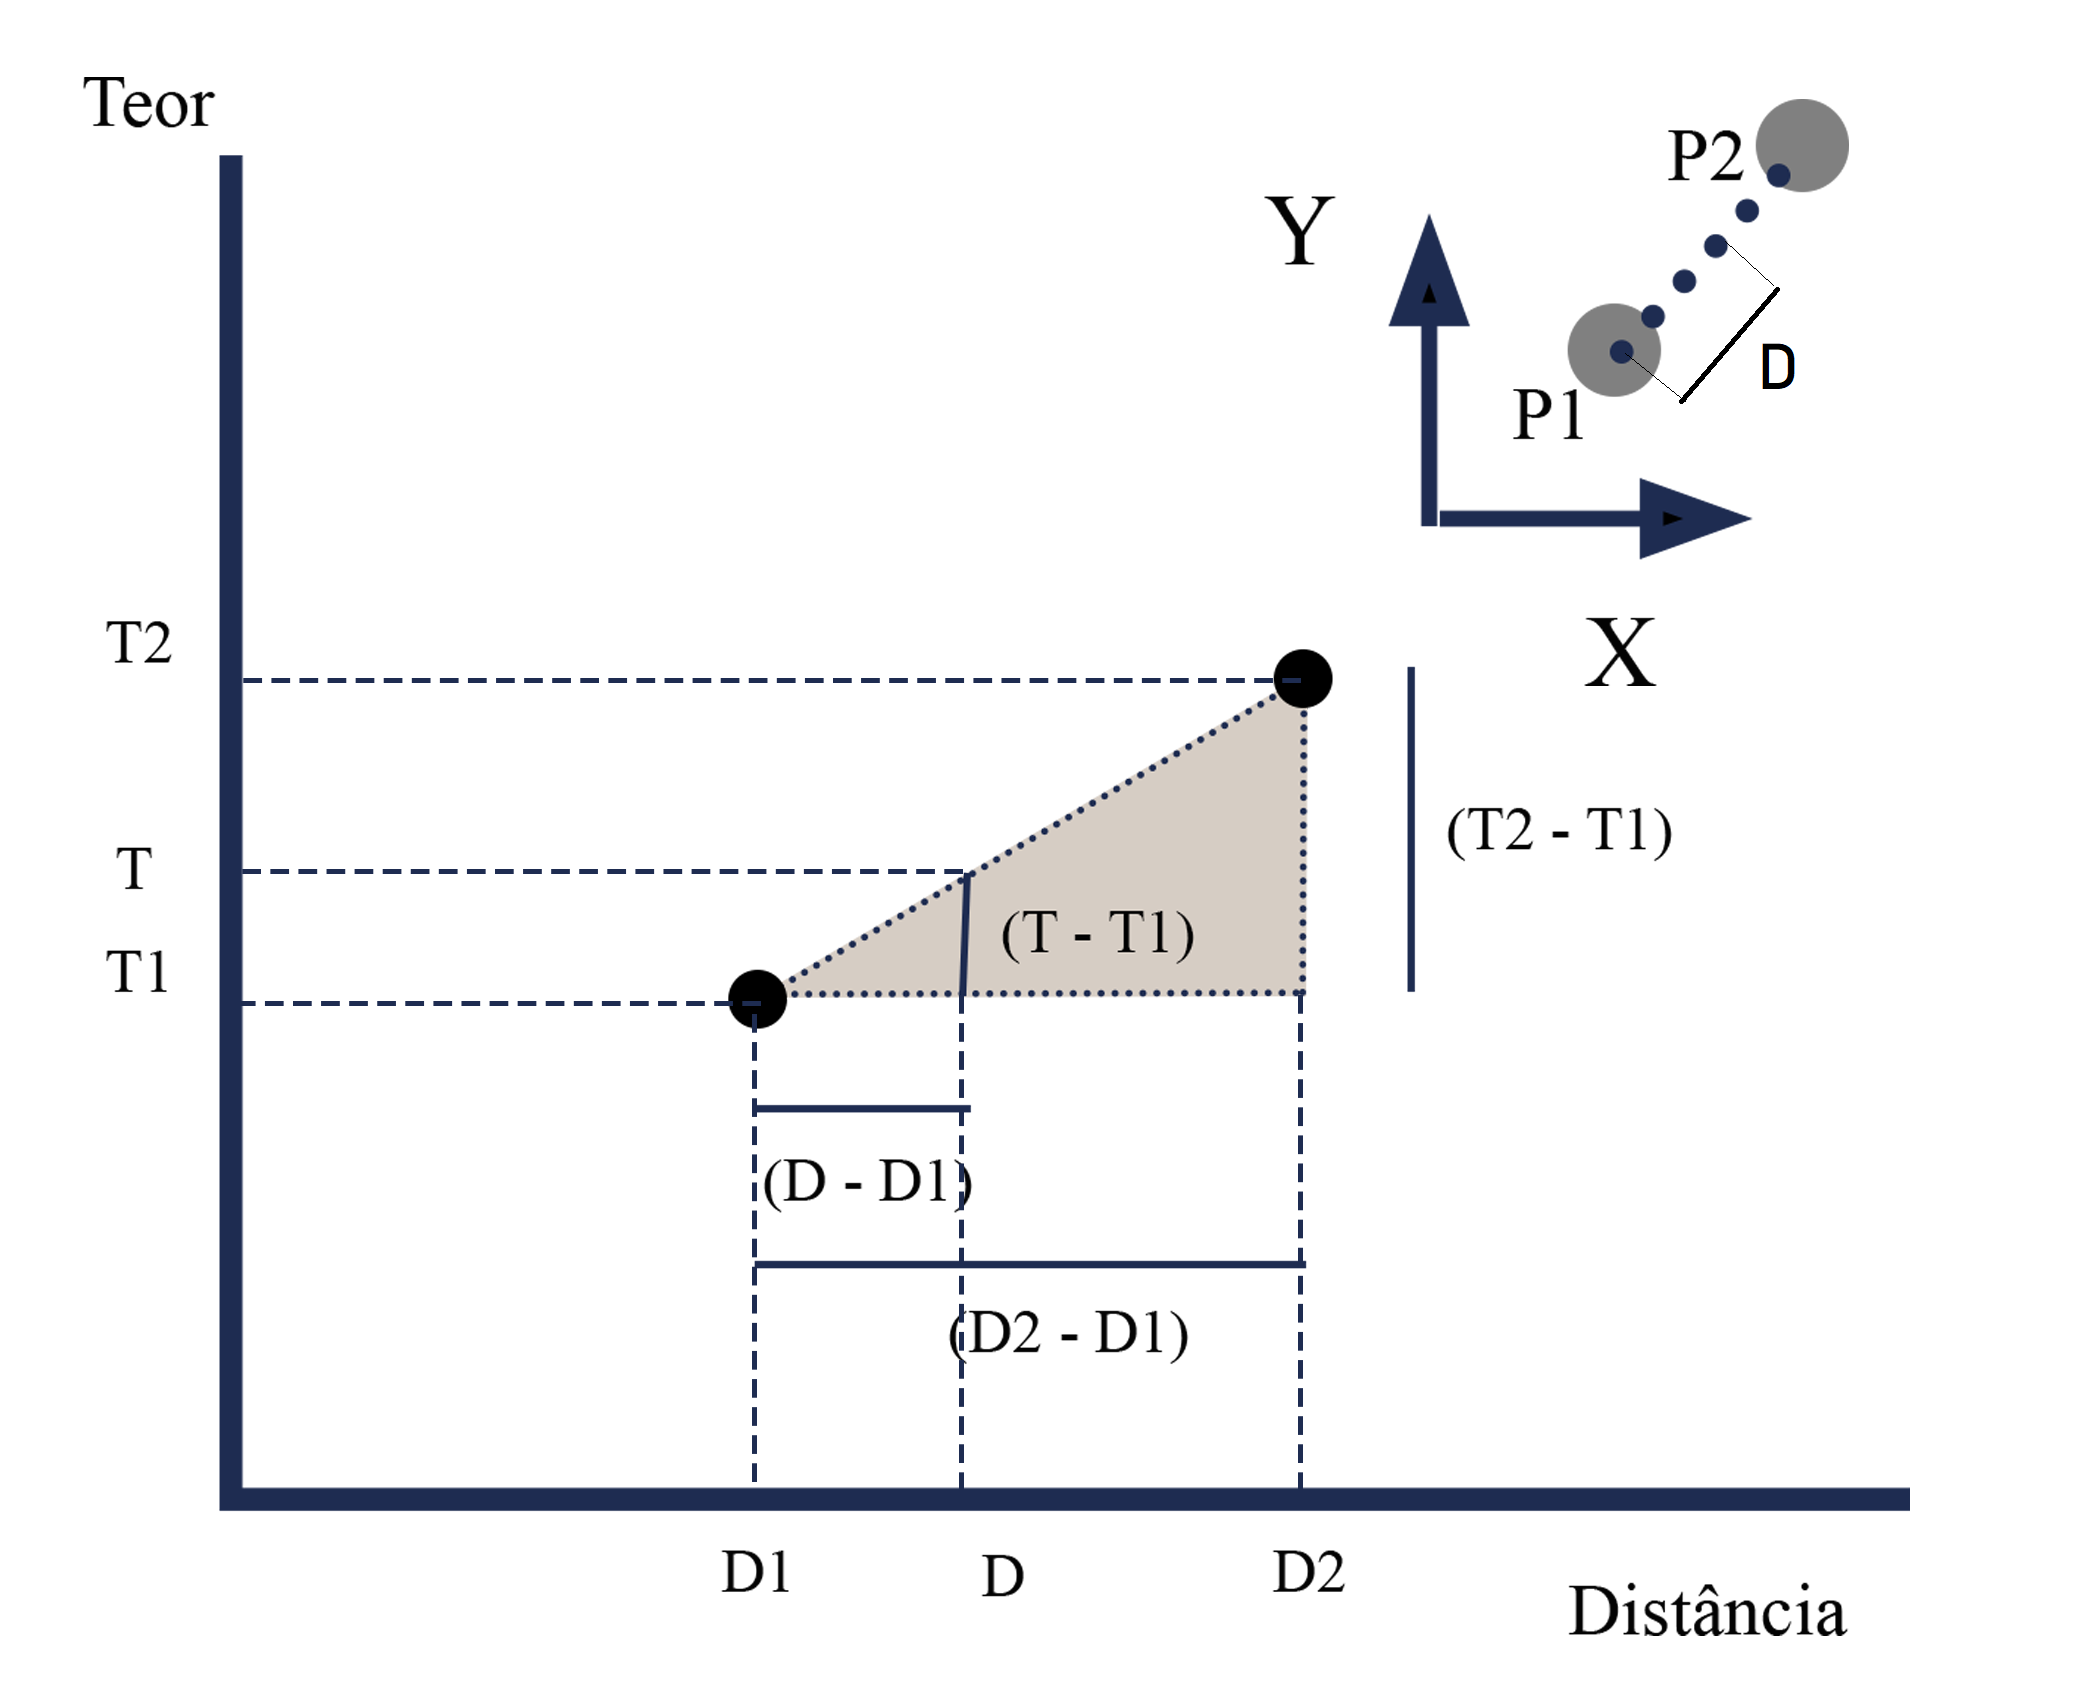
\includegraphics[scale=0.4]{./Capitulo_4/Gradual.png}	
	\caption{Princípio da mudança gradual de um teor para duas amostras no espaço $P1$ e $P2$, variação linear dos teores para uma distância $D$ considerada.}
	\label{mudgrad}
\end{figure}
\FloatBarrier

\subsection{Princípio dos pontos mais próximos} 

O princípio dos pontos mais próximos assume que o valor interpolado é igual ao valor da amostra mais próxima dele. Este processo também é chamado de \textbf{vizinho mais próximo}. Dado um conjunto de amostras no espaço $P = \{P_{1},P_{2},P_{3},...,P_{n},\}$ com propriedades $T = \{T_{1},T_{2},T_{3},...,T_{n},\}$, com respectivas posições espaciais segundo um eixo cartesiando $(x,y,z)$, o valor de uma propriedade $T_{0}$ para uma amostra $P_{0}$ no espaço assume o valor 

\begin{equation}\label{vizinhoprox}
T_{0} = T_{i} | i \rightarrow min(\| P_{0},P_{i}\|), \forall i\in [1,n]
\end{equation}

Em que $\| P_{0},P_{i}\|$ representa a distância euclidiana entre o par conjugado de pontos no espaço para $n$ amostras, $min()$ representa o mínimo valor. A figura \ref{mindist} apresenta o princípio dos pontos mais próximos. Cinco pontos amostrais são apresentados P1, P2, P3, P4 e P5. Como a distância mínima entre o ponto a ser amostrado P0 até o ponto amostral mais próximo é D2, T0 recebe o valor de T2. 

\FloatBarrier
\begin{figure}[!htpb]
	\centering
	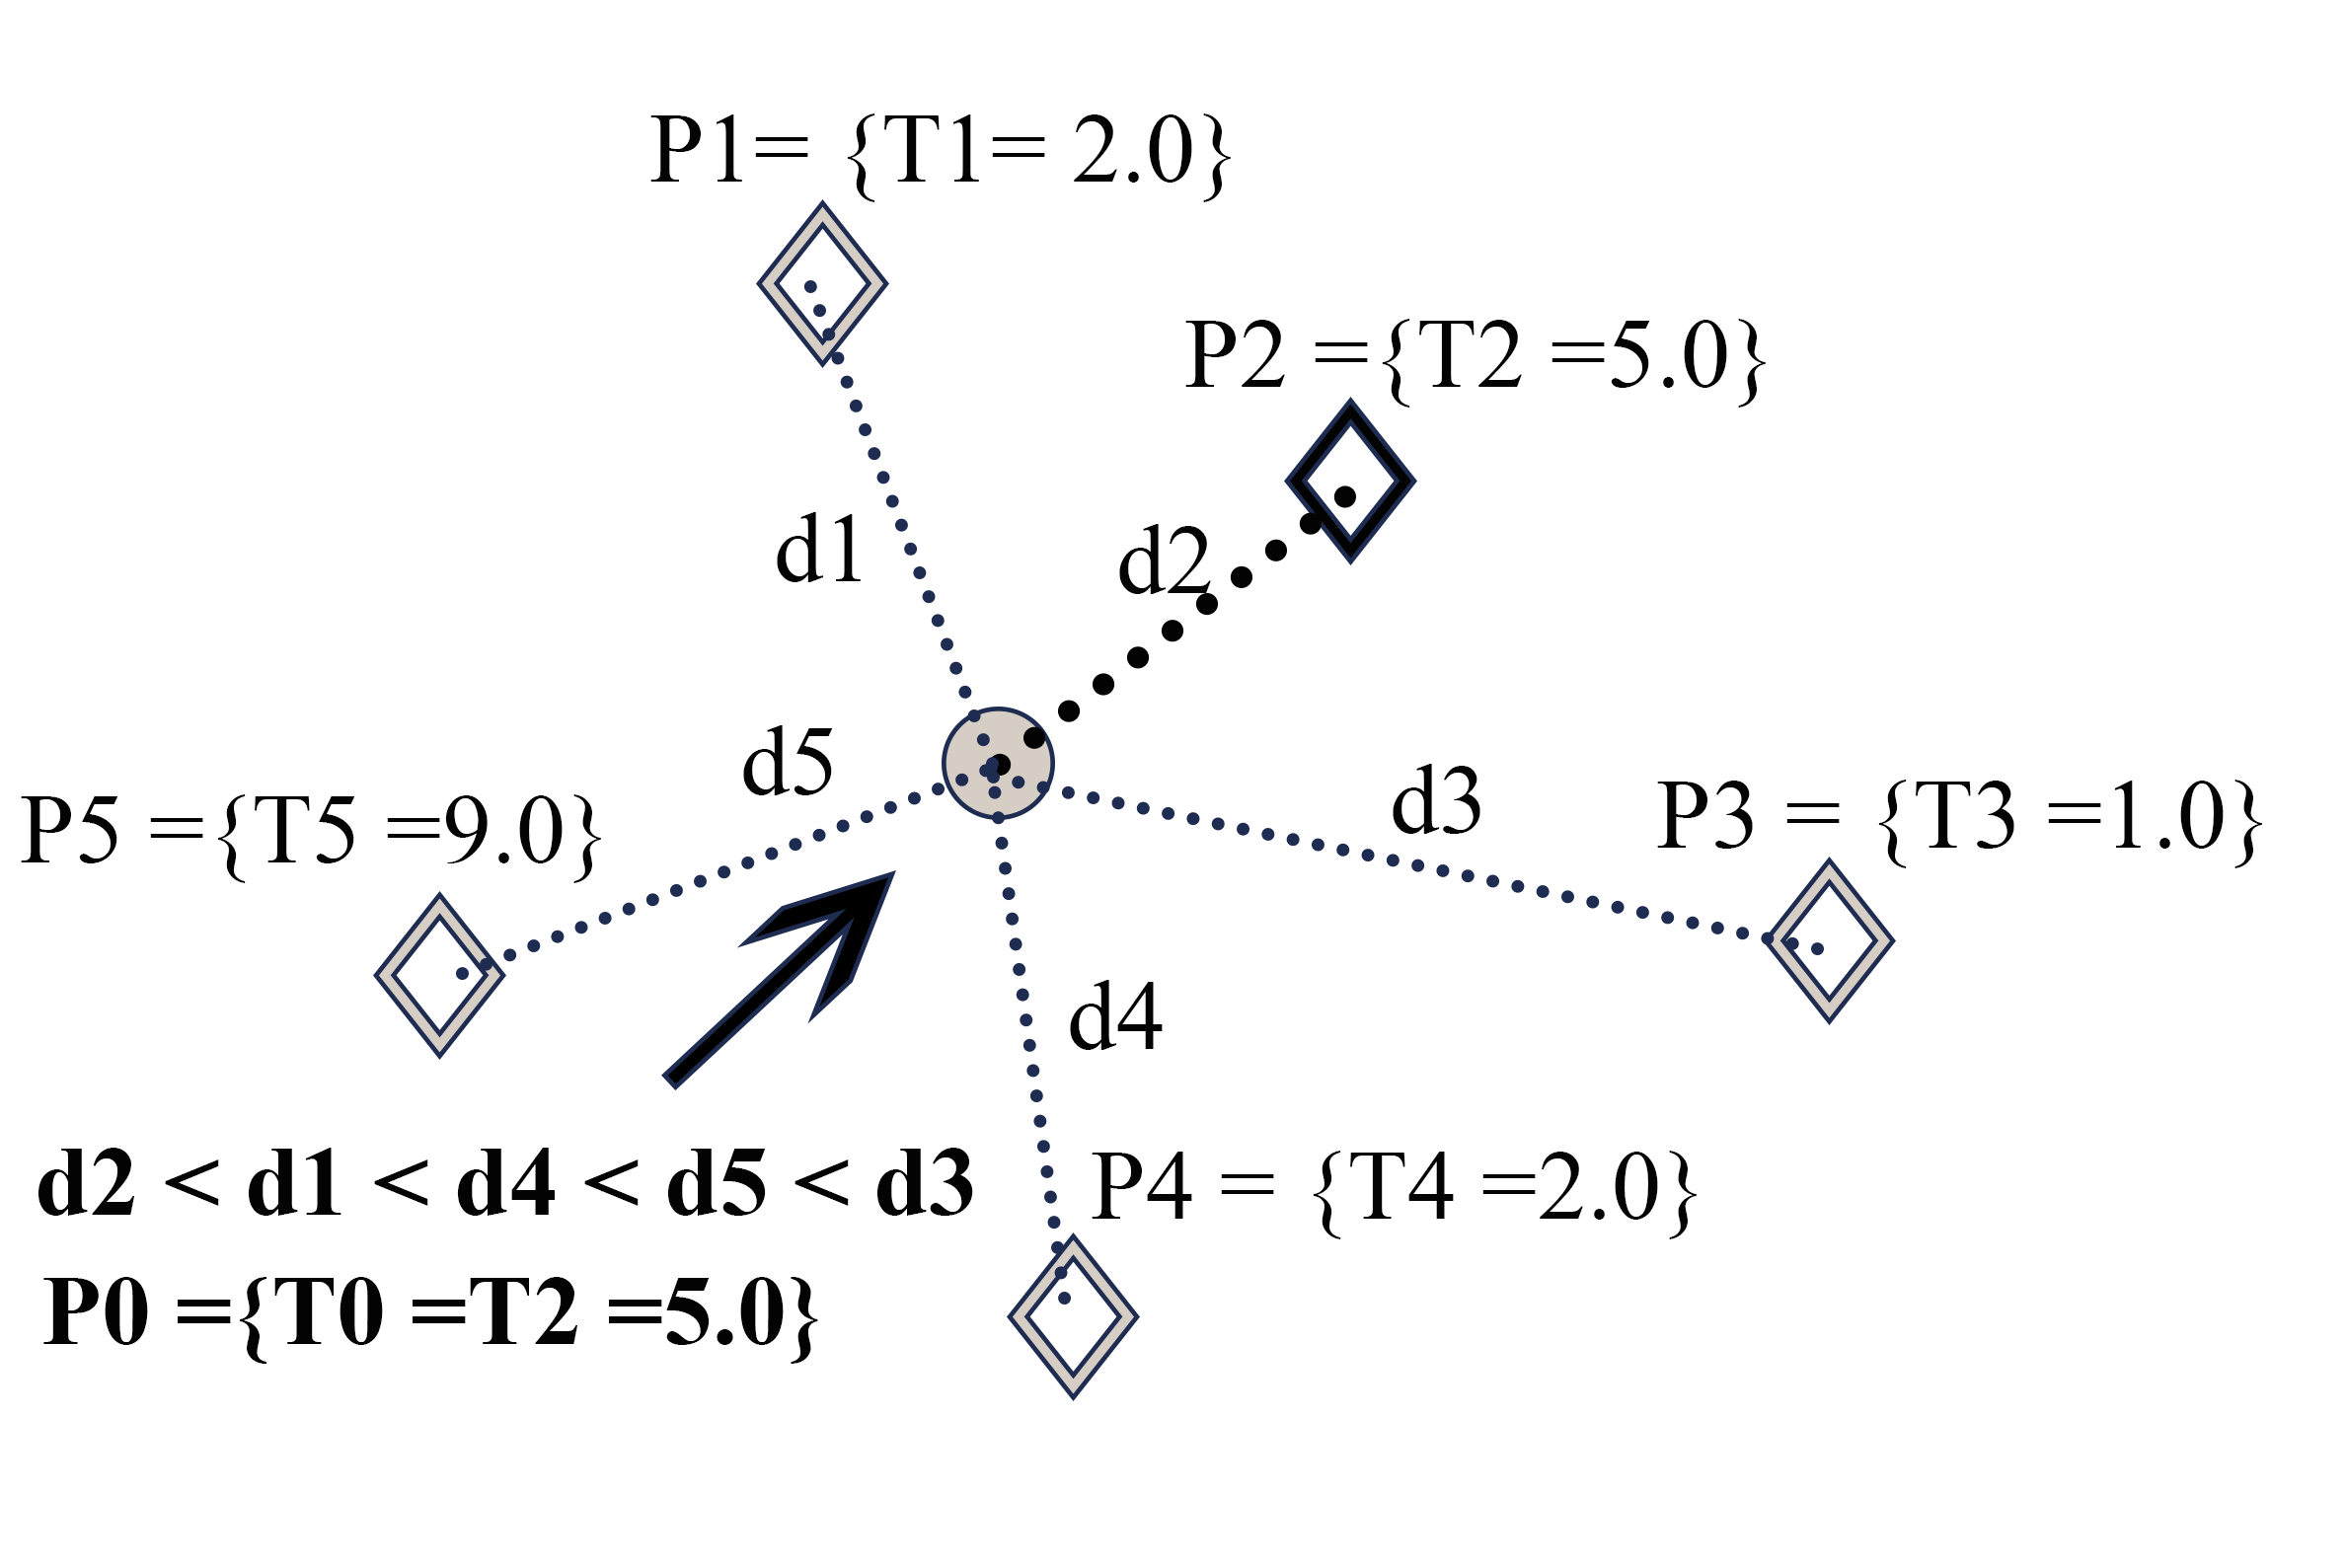
\includegraphics[scale=0.4]{./Capitulo_4/mindist.png}	
	\caption{Princípio dos pontos mais próximos. Conjunto de pontos amostrais P1, P2, P3, P4, P5 para um ponto amostral estimado P0. Como a menor distância euclidiana entre o ponto P0 é o ponto P2, assumimos que a propriedade T0 =T2. }
	\label{mindist}
\end{figure}
\FloatBarrier 

\subsection{Princípio da generalização}

Segundo critérios geológicos é possível realizar a extrapolação de uma dada propriedade segundo a continuidade do depósito mineral. Este princípio é justificado nas fases inciais de pesquisa para ajustar uma dada tendência das propriedades do depósito mineral. A figura \ref{extrap} demonstra a extrapolação do teor a partir do conhecimento de uma falha geológica entre os pontos amostrais $P1$ e $P2$. A partir da atitude da camada é estipulado uma variação segundo os teores extrapolados.

\FloatBarrier
\begin{figure}[!htpb]
	\centering
	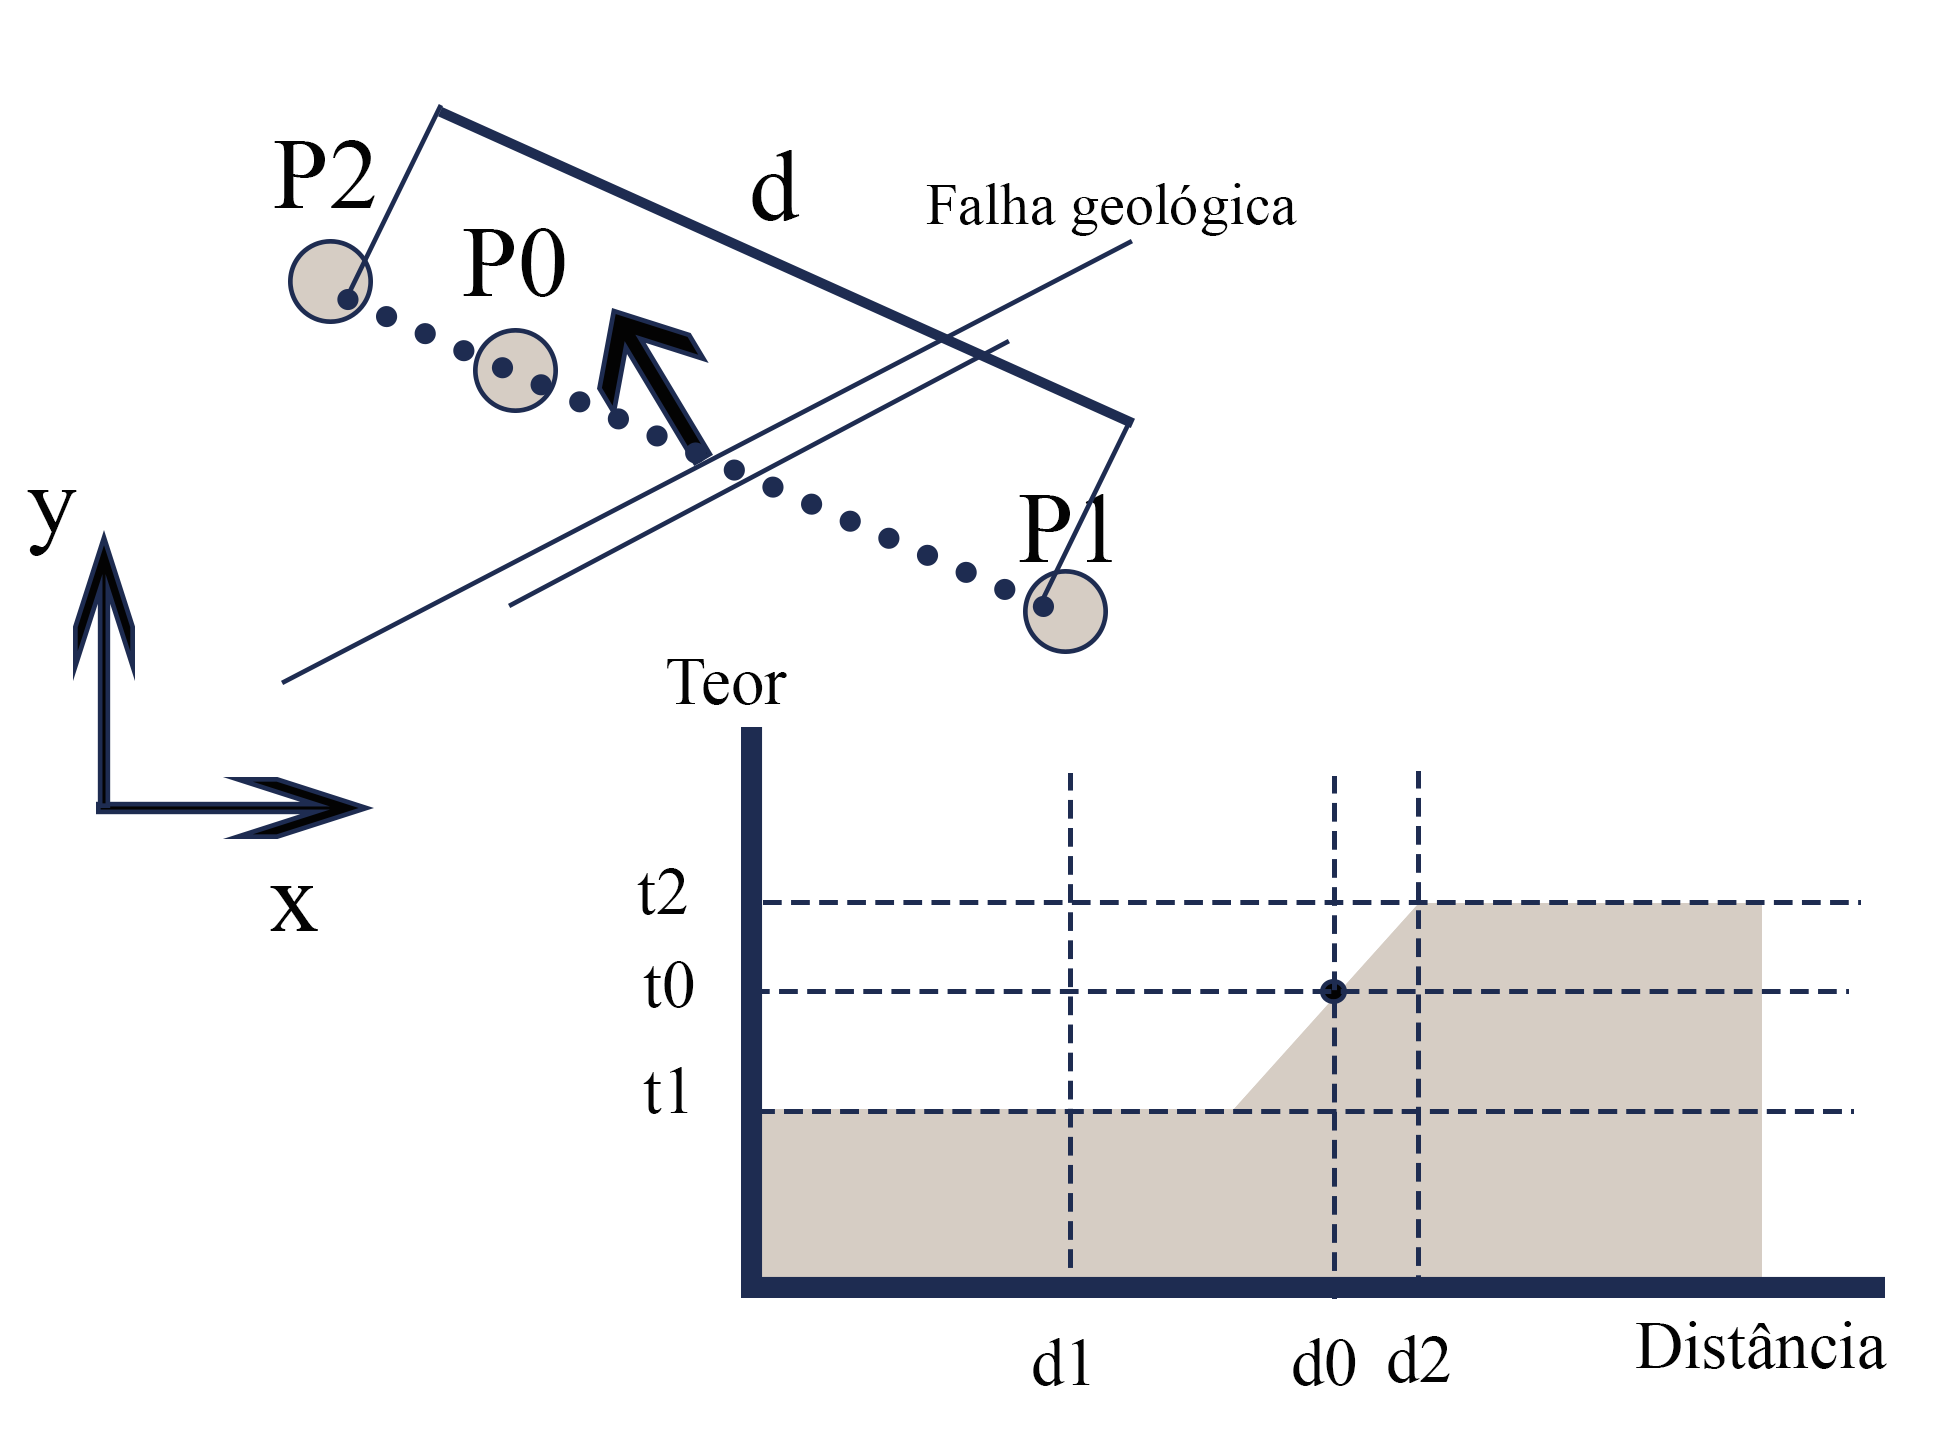
\includegraphics[scale=0.4]{./Capitulo_4/extrap.png}	
	\caption{Princípio da generalização e extensão dos teores a partir de um critério geológico. Falha geológica observada entre os pontos amostrais $P1$ e $P2$. Ponto estimado $P0$ é determinado a partir de diferenças entre os teorers e inclinação da camada. }
	\label{extrap}
\end{figure}
\FloatBarrier 

\section{Composição} 

Para realizar a análise geoestatística é necessário prover de amostras com mesmo \textbf{suporte}. Como testemunhos de sondagem podem representar fragmentos de tamanho distintos, é necessário realizar a \textbf{regularização} dos tamanhos das amostras. Isto significa que ao invés de tomarmos as propriedades referentes a apenas os fragmentos dos testemunhos de sondagem (litotipo, teores, propriedades físicas, etc.), tomamos a amostra como um valor de média ponderada entre os diversos tamanhos de fragmentos dos testemunhos. Observe a figura \ref{composicao}. Os framentos do testemunho de sondagem são respectivamente os valores $\{l_{1}, l_{2}, l_{3}, l_{4}\}$. Para consideramos este testemunho de sondagem como medidas representativas para a geoestatística consideramos duas composições de tamanho $\{C_{1}, C_{2}\}$, em que $\{x_{1}, x_{2}\}$ representam as respectivas partes dos fragmentos $\{l_{1}, l_{2}\}$ em $C_{1}$ . Se ${t_{1}, t_{2}, t_{3}, t_{4}}$ são propriedades aditivas como os teores dos fragmentos, podemos encontrar o valor da propriedade da composição $t_{C1}$ pela relação \eqref{eq:composition}

\begin{equation}\label{eq:composition}
t_{C_{1}} = \frac{(x_{1}/l_{1})t_{l_{1}} + (x_{2}/l_{2}) t_{l_{2}}}{(x_{1}/l_{1}) + (x_{2}/l_{2})}
\end{equation}

Em que $(x/l)$ representa a proporção de um dado fragemento dentro da composta. Podemos generalizar o caso da composição para n fragmentos de acordo com a relação \eqref{eq:composition2}

\begin{equation}\label{eq:composition2}
t_{C} = \frac{\sum_{i=0}^{n}(x_{i}/l_{i})t_{l_{i}} }{\sum_{i=0}^{n}(x_{i}/l_{i})}
\end{equation}

\FloatBarrier
\begin{figure}[!htpb]
	\centering
	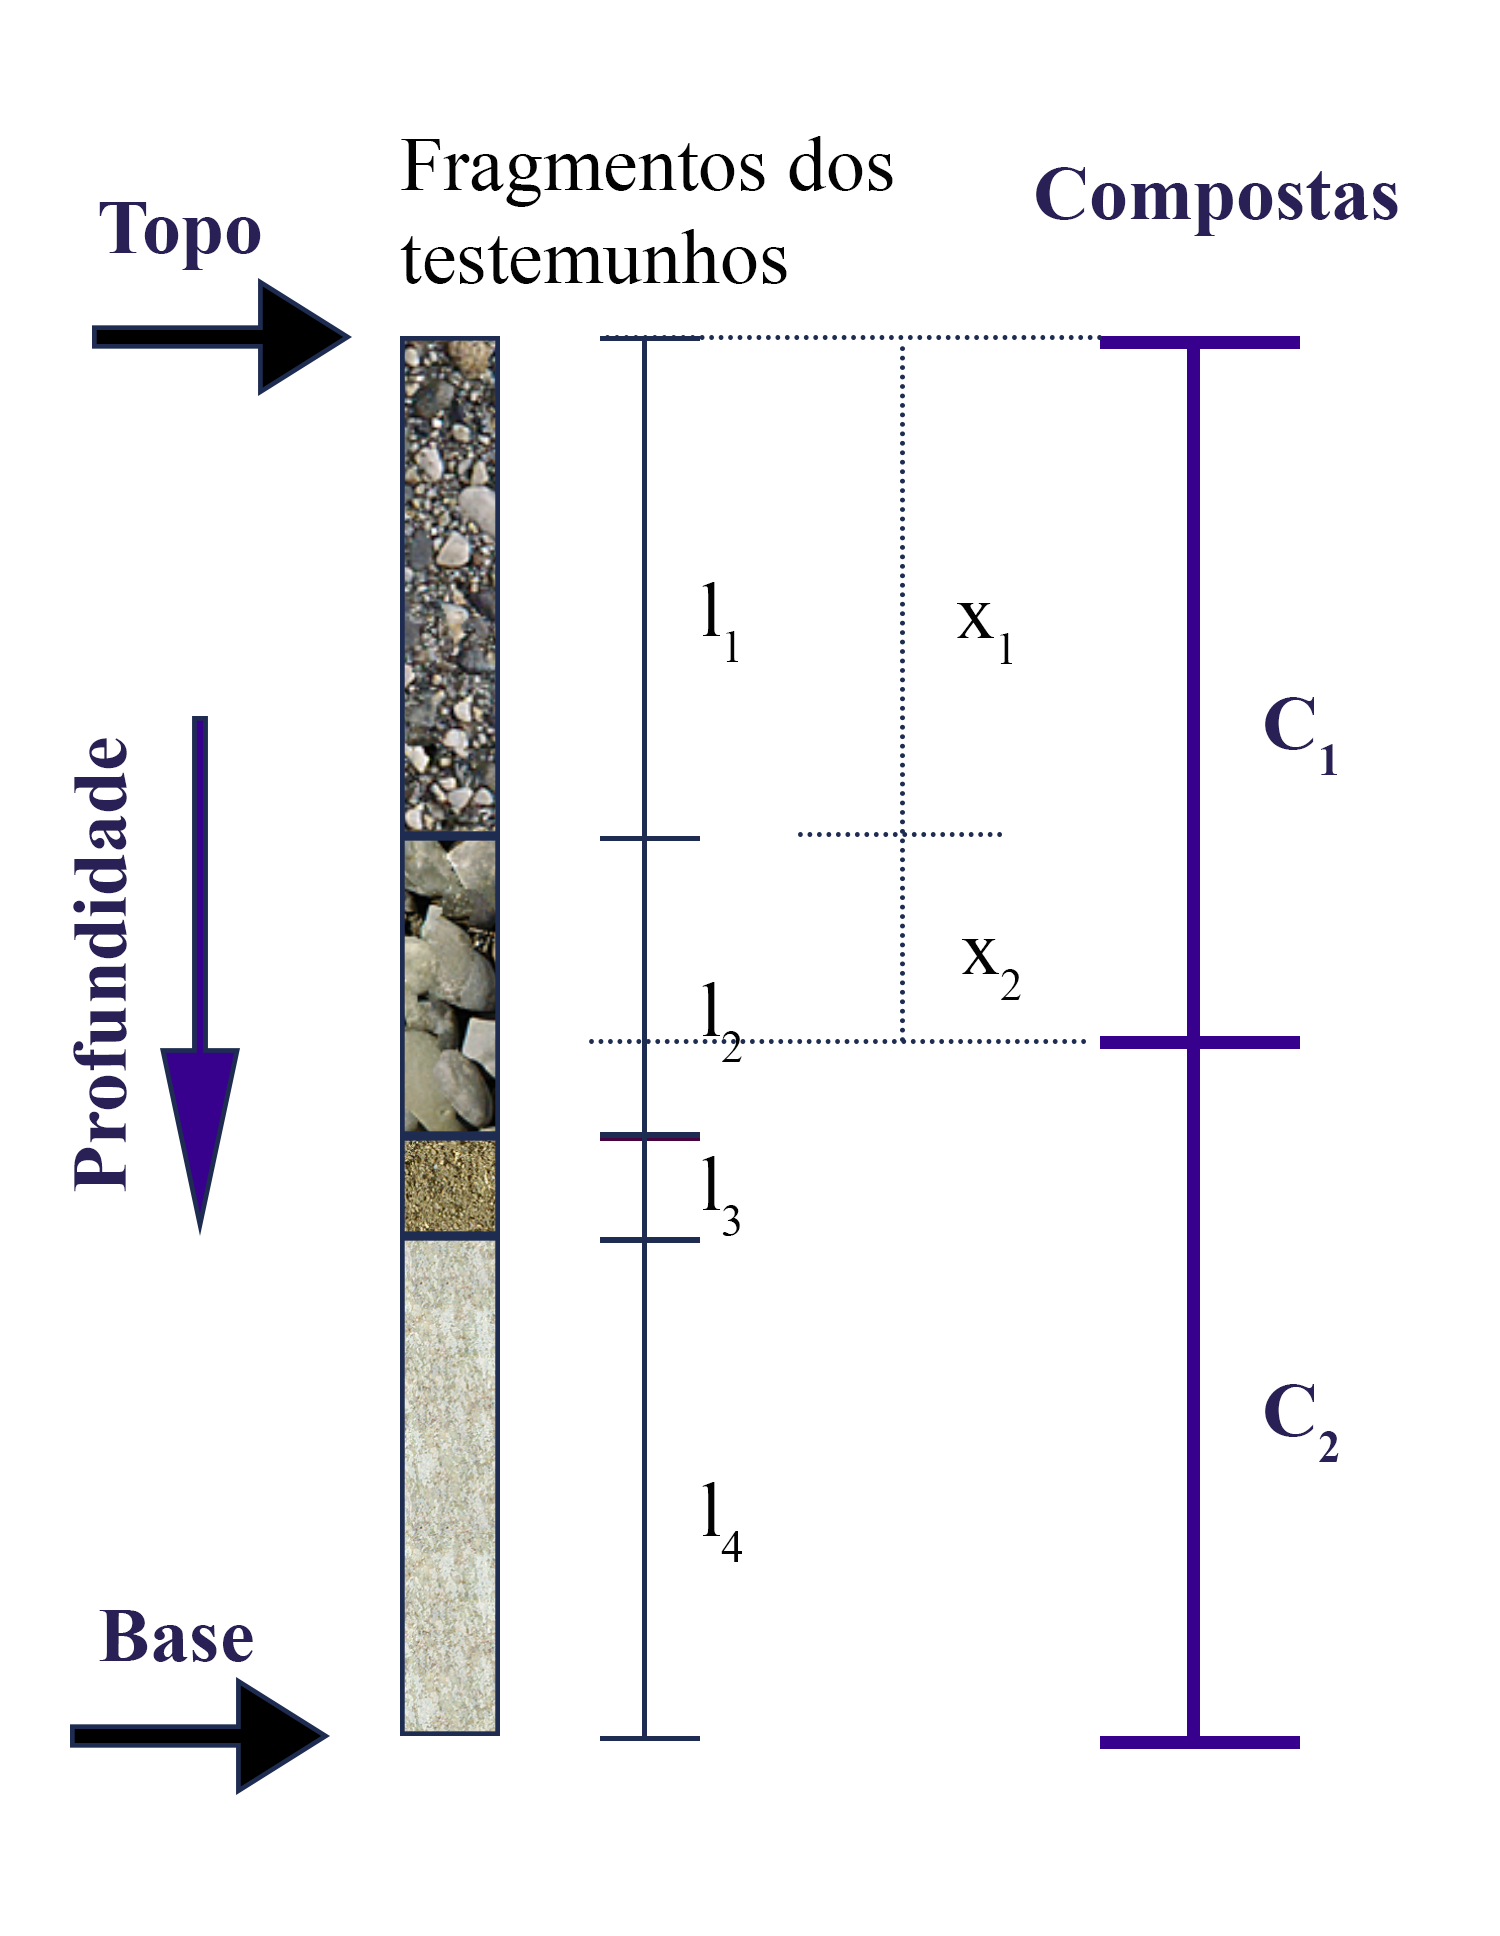
\includegraphics[scale=0.7]{./Capitulo_4/compostas.png}	
	\caption{Composição realizada em testemunho com 4 fragmentos $\{l_{1},l_{2},l_{3},l_{4}\}$ e tamanhos de composta igual  $\{C_{1},C_{2}\}$. $\{x_{1},x_{2}\}$ representam respectivamente as proporções dos fragmentos $\{l_{1},l_{2}\}$ dentro da composta $C_{1}$.  }
	\label{composicao}
\end{figure}
\FloatBarrier 

A escolha do tamanho da composição do testemunho geralmente está associada ao comprimento da manobra. Em alguns casos quando são realizados furos com manobras de tamanho diferenciado pode se optar pela moda dos valores de manobra. 

\begin{proposition}
	\textit{Devemos lembrar antes de realizar a composição de uma dada propriedade se ela pode ser caracterizada como uma variável aditiva, tal como teores e massas. A composição de testemunhos de sondagem considerando propriedades não aditivas deve ser realizada a partir dos estimadores adequados para as tendências centrais. Por exemplo, se considerarmos a velocidade de propagação de um pulso sísmo nos fragmentos, sabemos que a média correta de velocidade é a \textbf{harmônica} e não a média \textbf{aritmética}.}
\end{proposition} 

\section{Composição em seções verticais }

É comum durante o processo de estimativa, o geólogo realizar seções interpretadas de um depósito mineral, considerando os aspectos estruturais do depósito, o controle geológico entre outras características que formam um \textbf{modelo geológico}. Diferentemente de um \textbf{modelo estatístico} que prevê o conhecimento de variáveis aleatórias do depósito mineral,  o modelo geológico é uma representação dos diferentes litotipos dispostos no espaço, e nem sempre podem ser correlacionados com suas devidas propriedades. Para incorporar os valores das propriedades nas interpretações geológicas podemos fazer um "preenchimento" das seções a partir de valores médios obtidos nelas.  Este processo segue o princípio da generalização tomando o valor médio de uma seção interpretada como valor médio dos testemunhos contidos dentro daquela seção, ou daqueles bem próximos a seção interpretada. Observe a figura \ref{composicao2}, temos 6 compostas realizadas em furos $\{F1, F2, F3, F4, F5, F6\}$ correspondendo a área cinza da seção interpretada. Os valores de teores são respectivamente $\{t_{1},t_{2},t_{3},t_{4},t_{5}, t_{6}\}$ de comprimentos $\{l_{1},l_{2},l_{3},l_{4},l_{5}, l_{6}\}$

\FloatBarrier
\begin{figure}[!htpb]
	\centering
	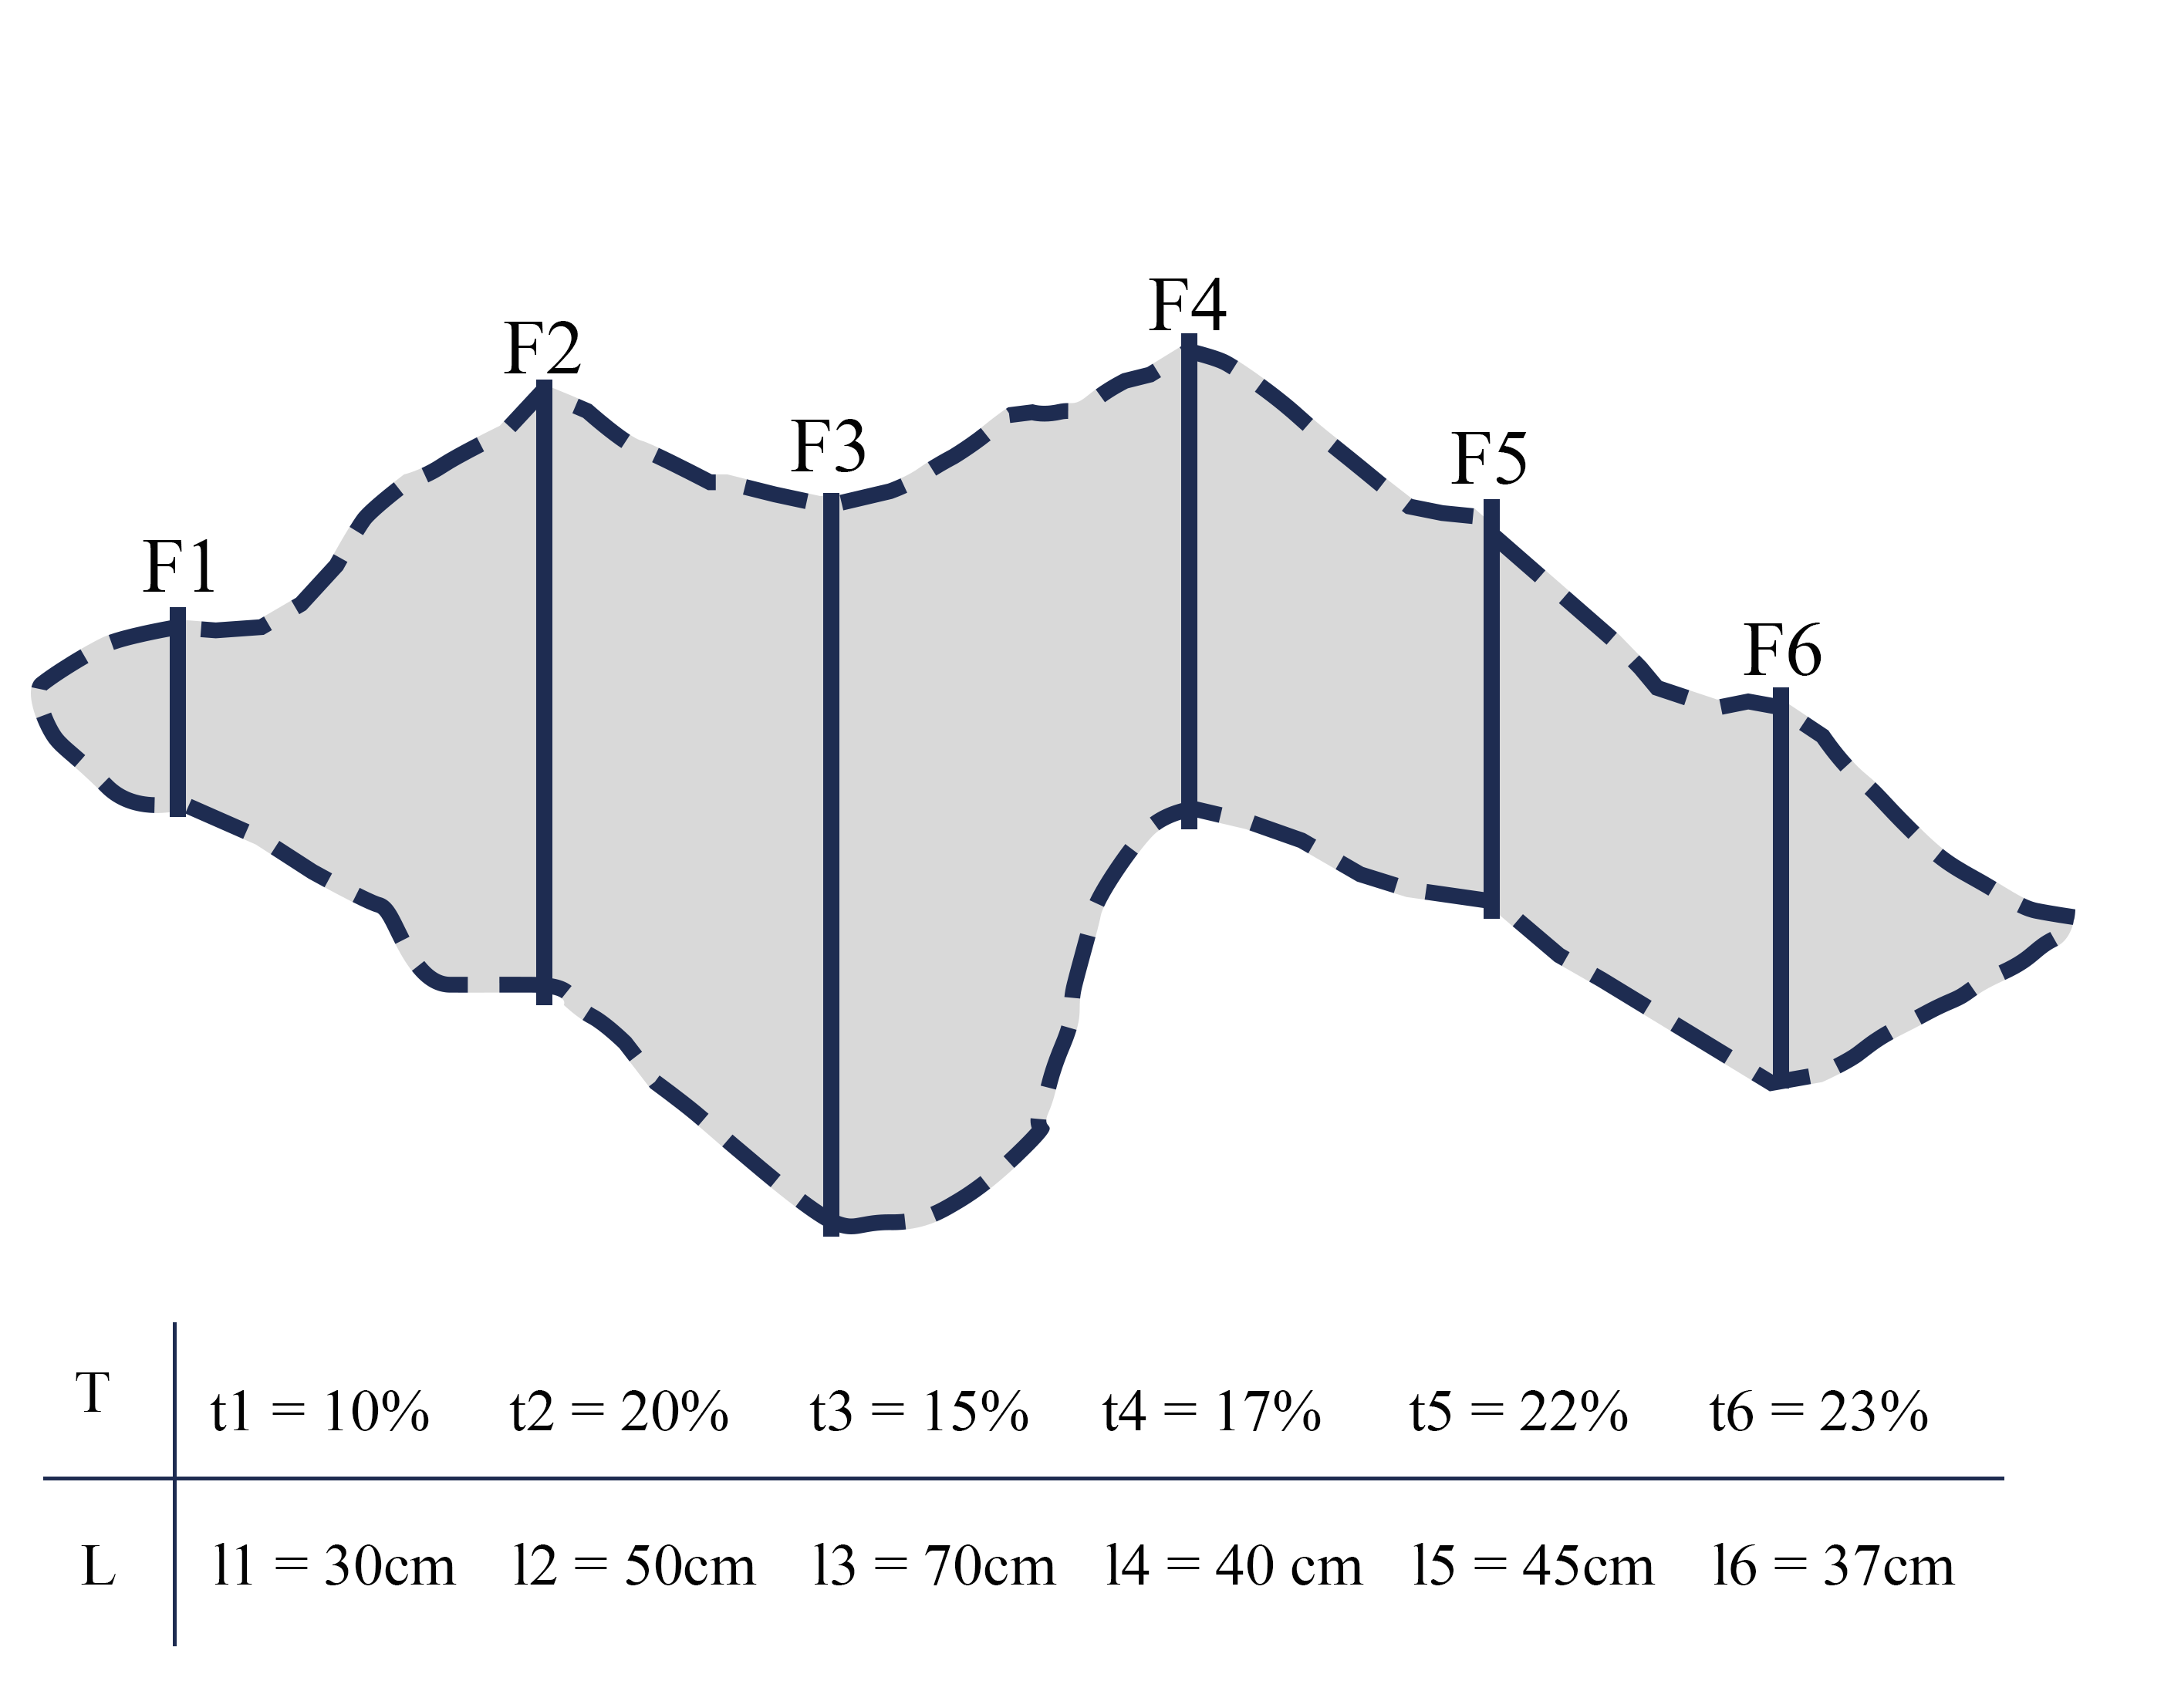
\includegraphics[scale=0.7]{./Capitulo_4/section_grade.png}	
	\caption{Composição realizada em testemunho com 4 fragmentos $\{l_{1},l_{2},l_{3},l_{4}\}$ e tamanhos de composta igual  $\{C_{1},C_{2}\}$. $\{x_{1},x_{2}\}$ representam respectivamente as proporções dos fragmentos $\{l_{1},l_{2}\}$ dentro da composta $C_{1}$.  }
	\label{composicao2}
\end{figure}
\FloatBarrier       

Para obtermos o valor médio da seção podemos realizar a seguinte operação de composição \eqref{composite_area}

\begin{equation} \label{composite_area} 
t_{C} = \frac{\sum_{i=1}^{6}t_{i}l_{i}}{\sum_{i=1}^{6}l_{i}} = \frac{10*30 + 20*50 + 15*70 + 17*40 + 22*45 + 23*37}{30+50+70+40+45+37}=17.91\%
\end{equation}

\section{Determinação de volumes} 

Um dos valores mais importantes obtidos na produção mineral é o volume do material a ser extraído, esse processo também é chamado de \textbf{cubagem}. A mineração consiste em movimentar um grande volume de rochas de diferentes litotipos. Infelizmente as informações obtidas das rochas são descritas apenas por amostras de pequeno volume e extensão, como em testemunhos de sondagem, durante as primeiras etapas da pesquisa mineral. Em alguns casos é possível obter trincheiras ou verificar as estruturas geológicas em painéis de mina subterrânea. Estes volumes estimados são geralmente obtidos pela interpretação geológica de um profissional engenheiro de minas ou geólogo, capaz de entender os processos de gênese destes depósitos minerais. Uma das alternativas consiste em realizar seções verticais contendo informações dos furos de sondagem e realizar a extrapolação de volumes a partir da extensão das áreas interpretadas. Dado uma série de seções $S$ de área $A$, o volume entre seções pode ser obtido a partir da equação \eqref{volumes}

\begin{equation} \label{volumes}
	V = \sum_{i=1}^{n-1}D_{i}(A_{i} + A_{i+1})/2
\end{equation}

Onde $D_{i}$ é a distância entre as seções $A_{i}$ e $A_{i+1}$ para n seções consideradas. Os volumes obtidos pelas seções das pontas é obtido a partir de extrapolação dado uma distância considerada aceitável pelo geólogo, baseando-se em critérios de continuidade. A figura \ref{extrap} apresenta a interpolação realizada a partir da interpretação geológica das seções e extrapolação destas para obtenção do volume.

\FloatBarrier
\begin{figure}[!htpb]
	\centering
	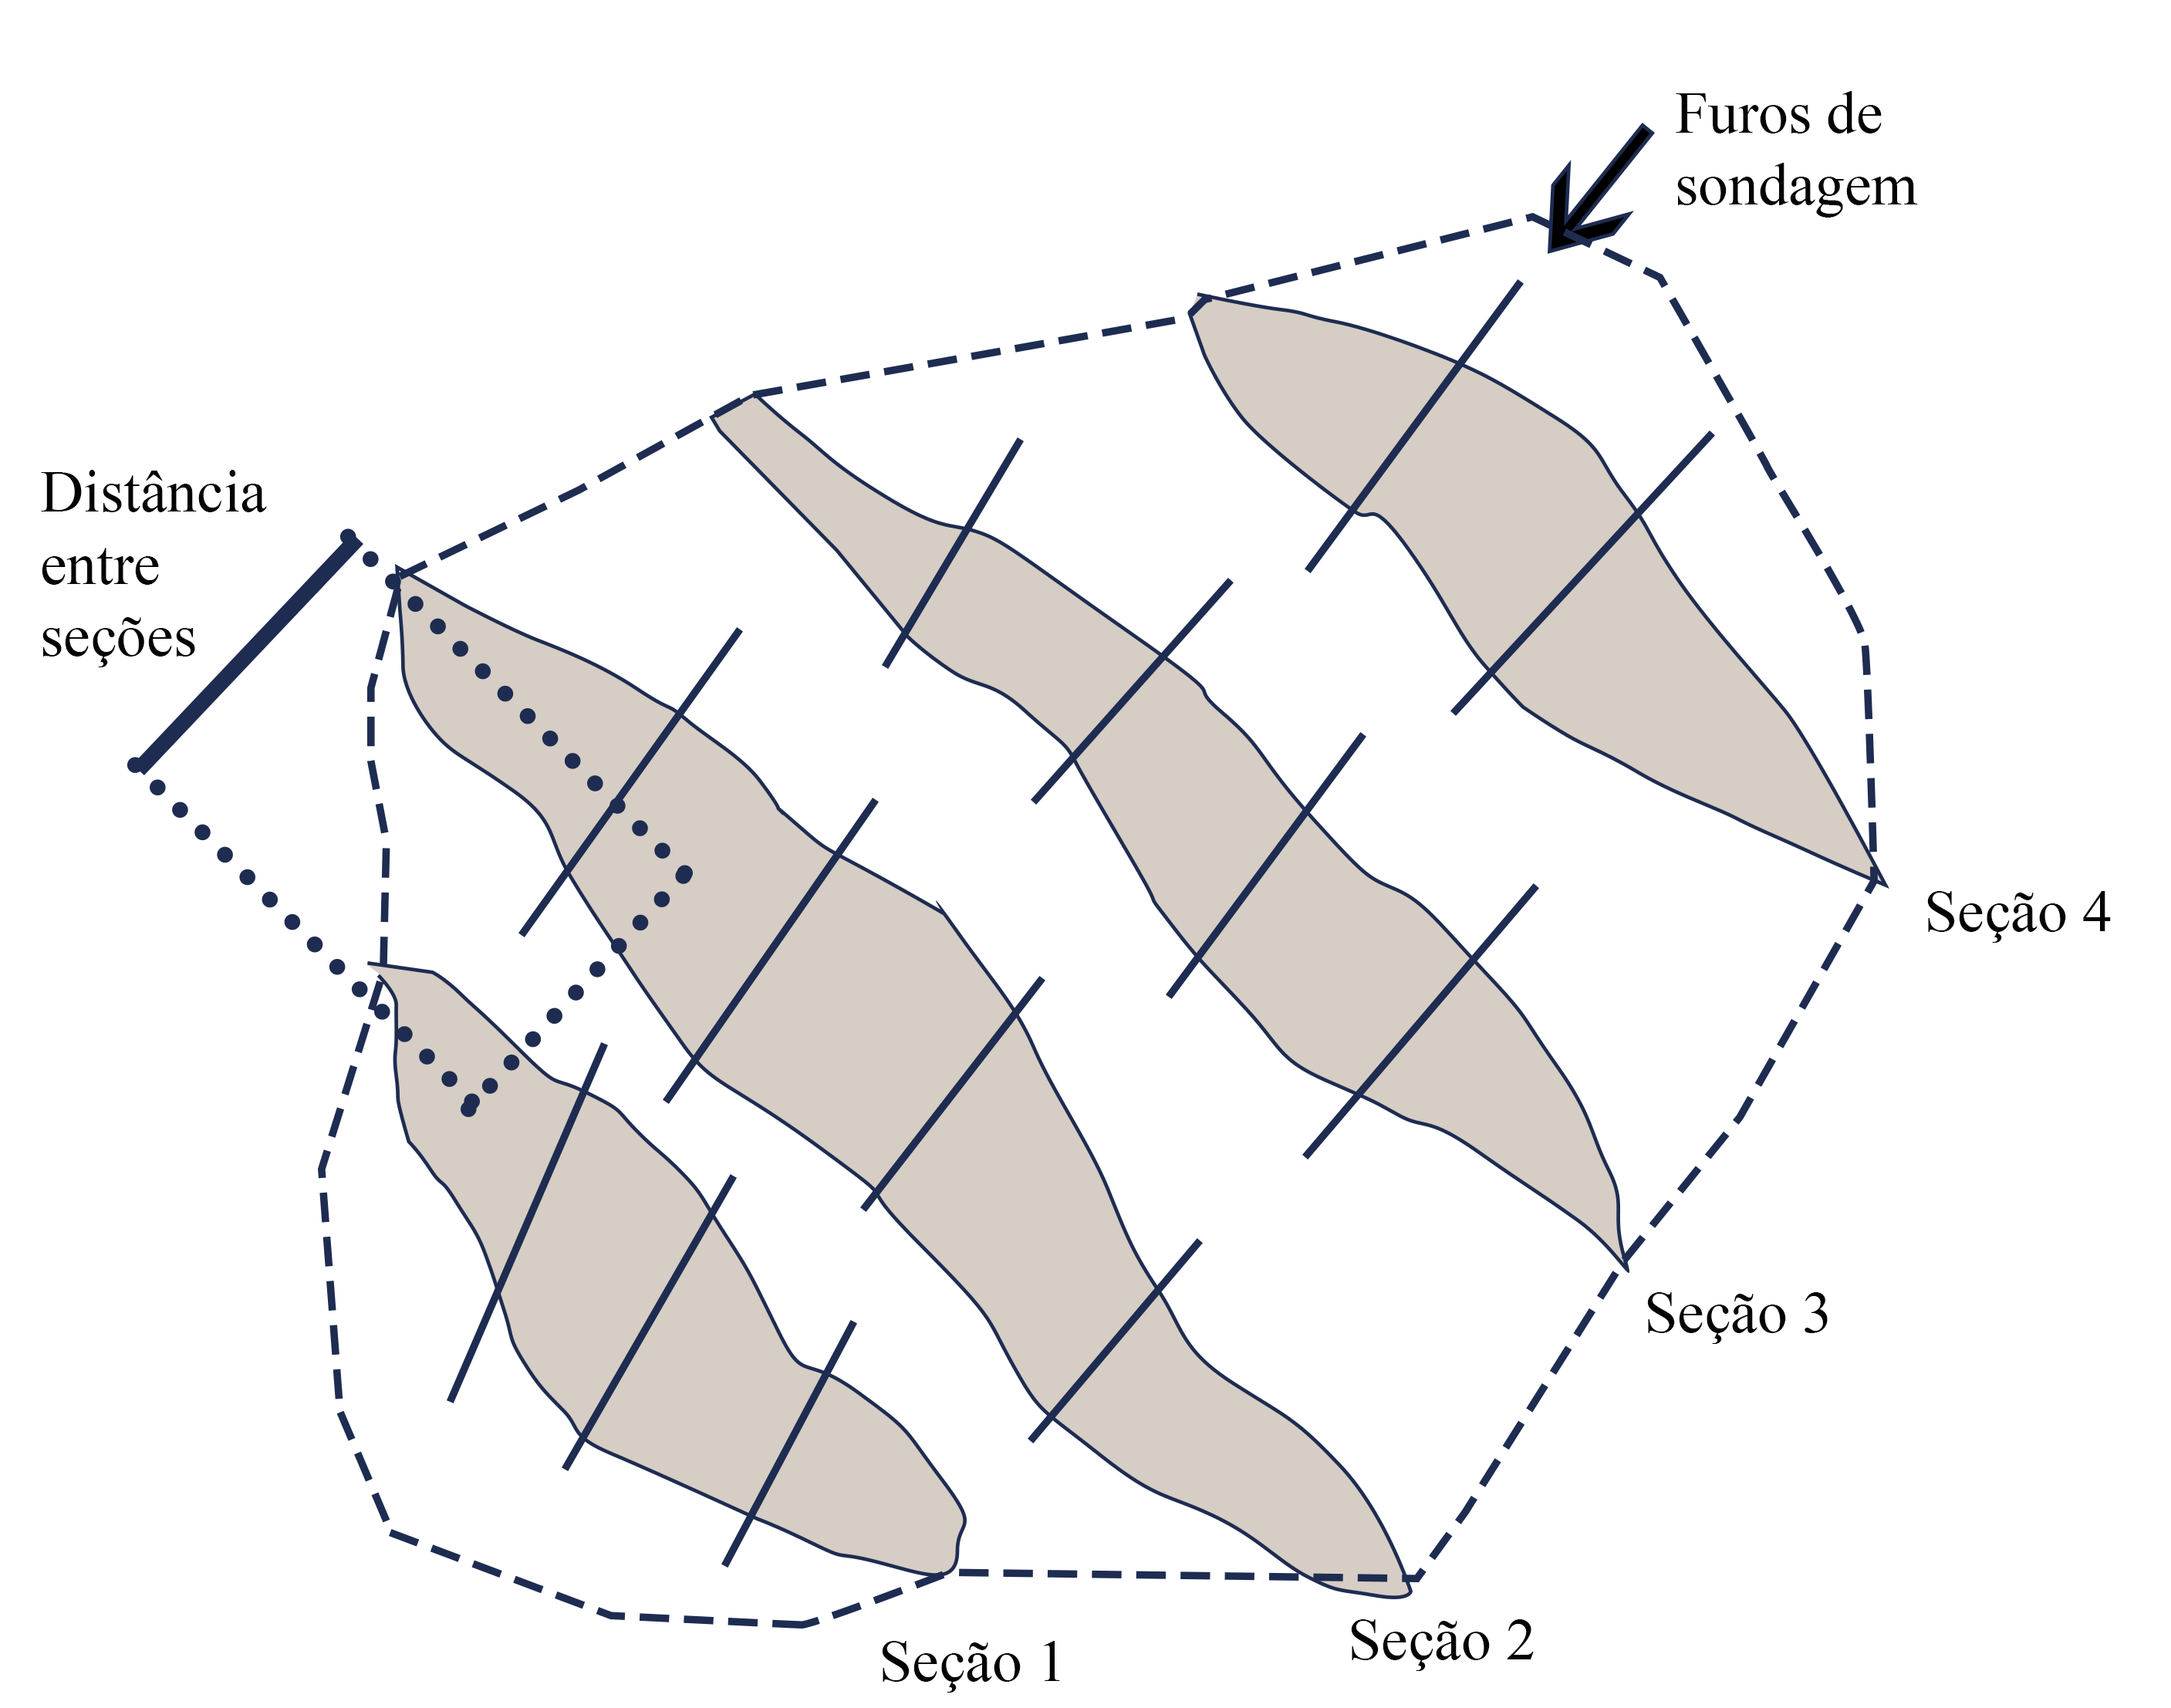
\includegraphics[scale=0.4]{./Capitulo_4/volumes.png}	
	\caption{Obtenção dos volumes dos corpos geológicos a partir de extrapolação de seções verticais interprestadas. Cinco seções consideradas e os respectivos furos de sondagens utilizados para interpretar os volumes. }
	\label{extrap}
\end{figure}
\FloatBarrier 

\begin{proposition}
	\textit{Apesar de ser um método antigo de avaliação de volumes, as interpretações de seções ainda são utilizadas na prática. Apesar da dificuldade operacional deste método com a digitalização de seção por seção, permite a geólogos e engenheiros de minas incorporarem informações importantes para o modelo, como adição de estruturas geológicas, possíveis zonas de alteração, entre outras características típicas do depósito analisado. Métodos recentes como a \textbf{modelagem implícita} auxiliam muito na velocidade de produção dos modelos, mas geralmente precisam de um cuidado maior ao incorporar outras informações após serem gerados}
\end{proposition}

\section{Inverso do quadrado da distância - IQD} 

Um dos interpoladores mais antigos conhecidos é o uso do inverso do quadrado da distância. A justificativa da utilização deste ponderador é que muitos problemas físicos ocorrem a partir de leis de decaimento quadráticas. O uso de outras potências também pode ser utilizado, mas a medida que esta potência cresce, os valores mais próximos das regiões estimadas tendem a ser mais valorizados, reduzindo a suavização da interpolação. Dada uma propriedade $t$ como  o teor de uma amostra $P$, situada a uma distância $d$ do centroide de uma célula estimada, a média estimada desta célula pode ser calculada pela equação \eqref{iqd_form}: 

\begin{equation}\label{iqd_form} 
t_{m} = \frac{\sum_{i=1}^{n}\frac{1}{d_{i}^{p}}t_{i}}{\sum_{i=1}^{n}\frac{1}{d_{i}^{p}}}
\end{equation} 

Em que $p$ é o grau do polinômio considerado para $n$ amostras situadas nas redondezas da célula estimada. Se o número de amostras é grande, o cálculo dos ponderadores geralmente é realizado apenas com os valores mais próximos, para isto utilizando um algoritmo que filtre segundo a proximidade das amostras da célula estimada. Observe a figura \ref{IQD}.

\FloatBarrier
\begin{figure}[!htpb]
	\centering
	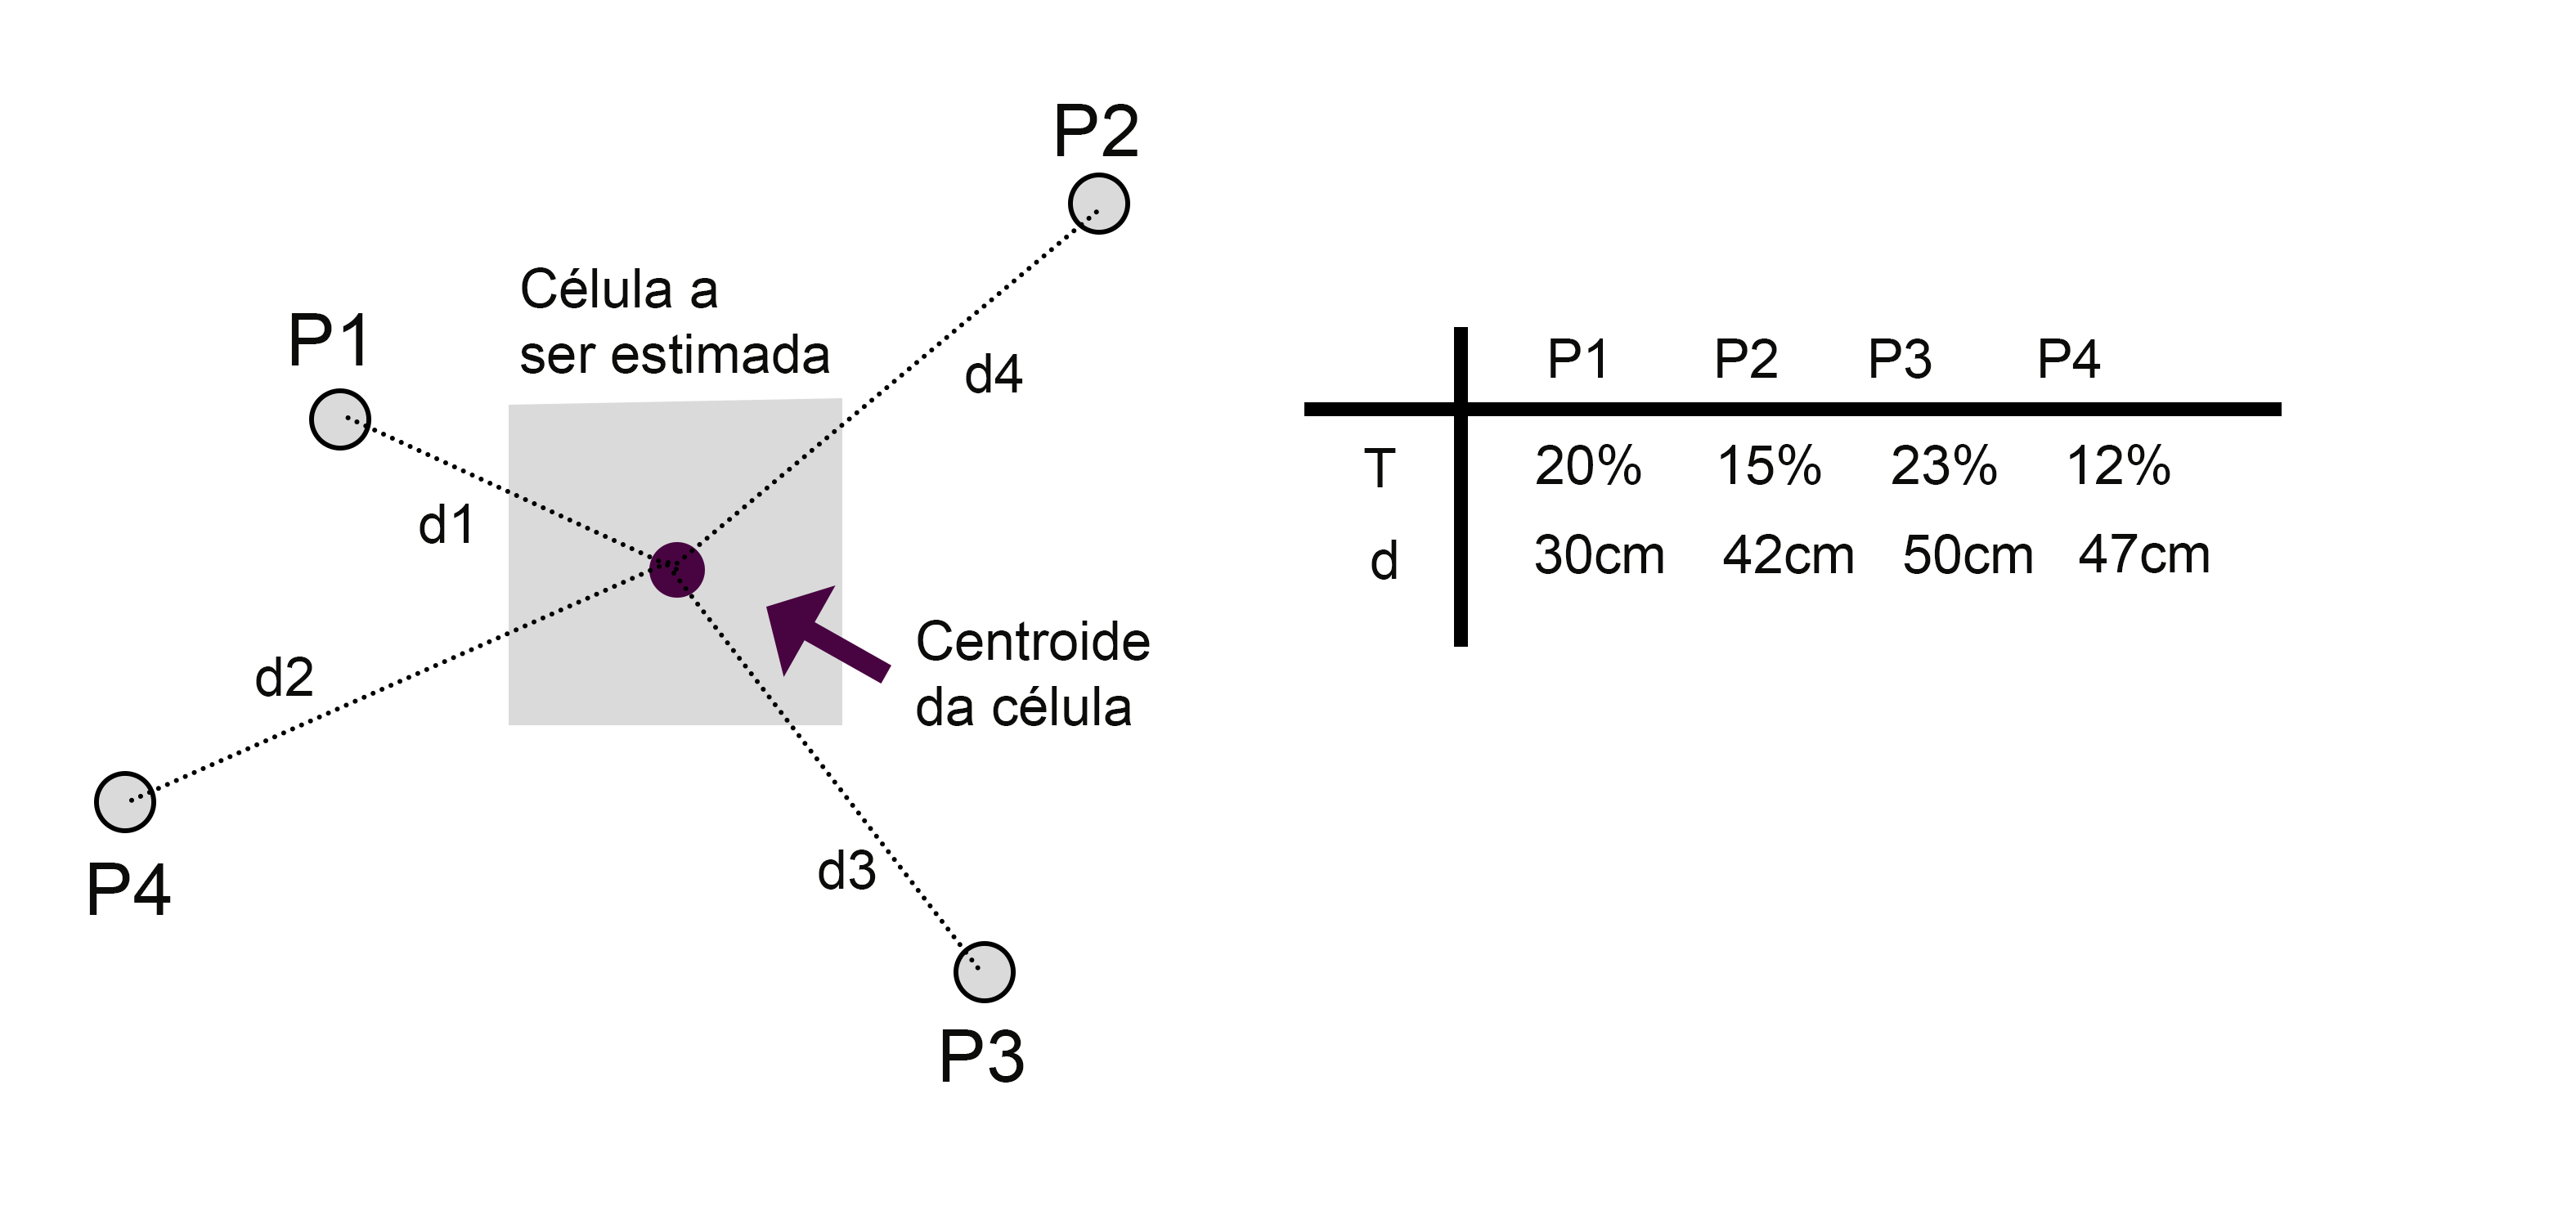
\includegraphics[scale=0.8]{./Capitulo_4/IQD.png}	
	\caption{Obtenção dos volumes dos corpos geológicos a partir de extrapolação de seções verticais interprestadas. Cinco seções consideradas e os respectivos furos de sondagens utilizados para interpretar os volumes. }
	\label{IQD}
\end{figure}
\FloatBarrier 

 Para 4 pontos mais próximos da célula estimada, temos respectivamente os valores de teor $(T)$ e a distância ao centroide da célula. Desta forma podemos calcular o valor médio da célula a partir de \eqref{calc_iqd_exp}

\begin{equation}\label{calc_iqd_exp}
t_{m} = \frac{1/(30^{2})20 + 1/(42^{2})15 + 1/(50^{2})23 + 1/(47^{2})12 }{1/(30^{2}) + 1/(42^{2}) + 1/(50^{2}) + 1/(47^{2}) } =17,92\%
\end{equation}

\section{Tesselação de Delunay} 

A interpolação espacial pode ser realizada a partir da \textbf{tesselação de Delunay}, dividindo o espaço entre as amostras em triângulos. Cada amostra é univocamente ligada a dois pontos mais próximos, sendo esta uma solução geométrica única. Os valores médios de cada triângulo é obtido a partir da média ponderada entre os tamanhos da composta e os valores das propriedades. Dado três pontos $\{ P_{1}, P_{2}, P_{3} \}$ com respectivos valores de teor $\{ t_{1}, t_{2}, t_{3} \}$ e comprimentos $\{ l_{1}, l_{2}, l_{3} \}$. O valor médio de cada triângulo pode ser obtido a partir de \eqref{pondtriang}

\begin{equation} \label{pondtriang} 
	t_{m} = \frac{t_{1}l_{1} + t_{2}l_{2} + t_{3}l_{3} }{l_{1} + l_{2} + l_{3}}
\end{equation}

Observe a figura \ref{tesselacao}. Estão dispostas sete amostras no espaço formando os triângulos de Delunay, e o triângulo $\{P_{1}, P_{2}, P_{3}\}$ está destacado.

\FloatBarrier
\begin{figure}[!htpb]
	\centering
	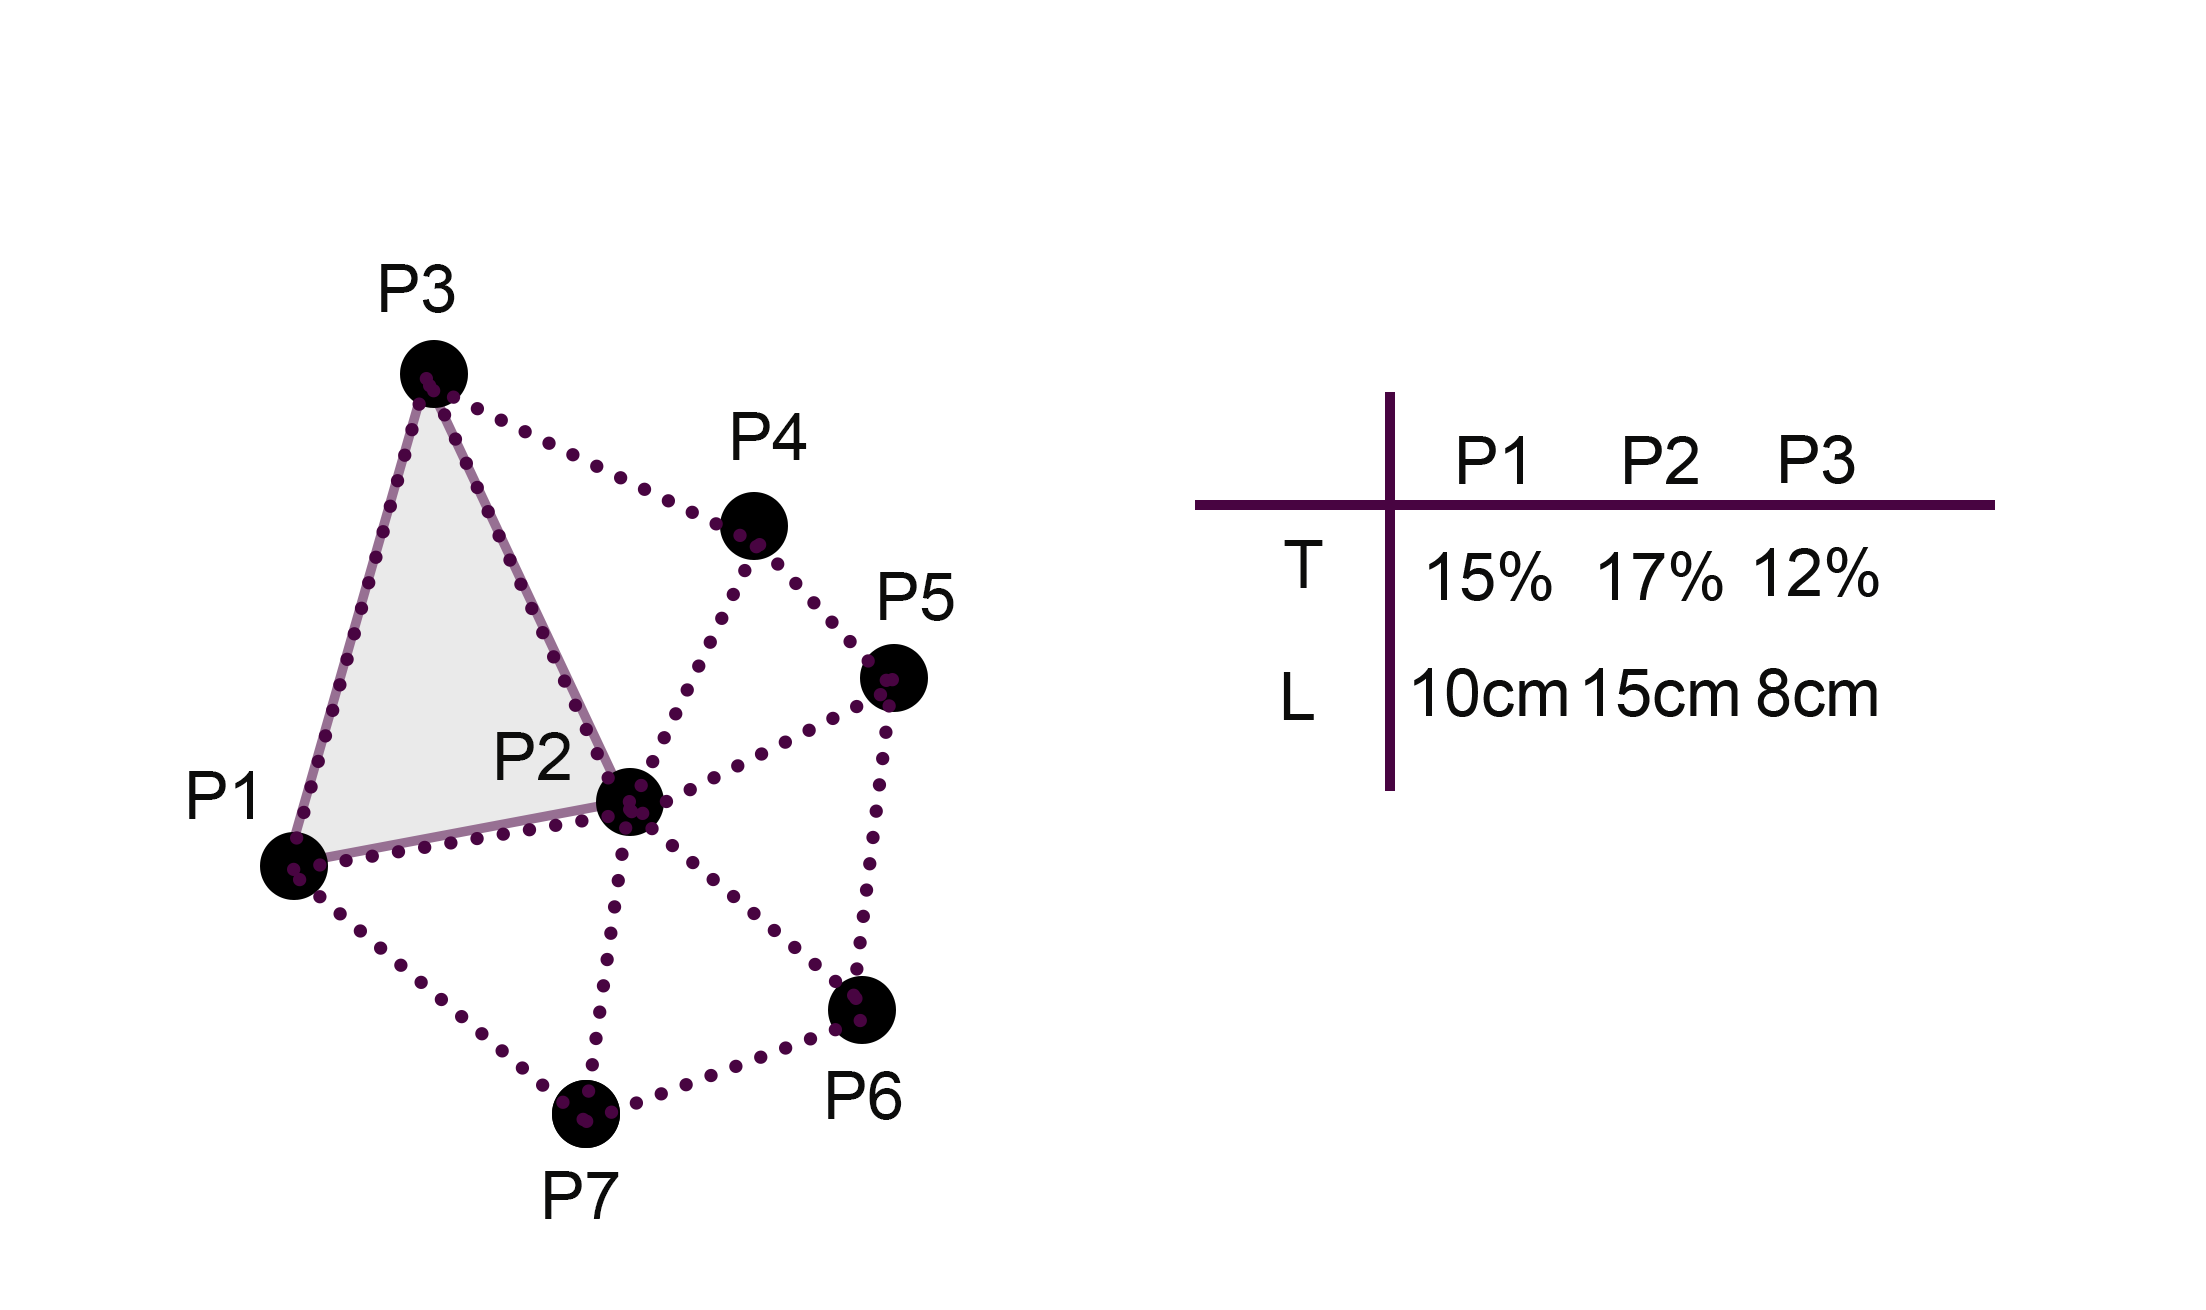
\includegraphics[scale=0.8]{./Capitulo_4/tesselacao.png}	
	\caption{Valor médio obtido em um triângulo de Thiessen. 3 pontos amostrais $\{P_{1},P_{2},P_{3}\}$, com valores de teor $\{t_{1},t_{2},t_{3}\}$. }
	\label{tesselacao}
\end{figure}
\FloatBarrier 

 Considerando $\{t_{1}, t_{2}, t_{3}\}$ os teores relativos a cada amostra, e $\{l_{1}, l_{2}, l_{3}\}$ o tamanho das compostas. Podemos calcular o valor do teor médio como

\begin{equation}
	t_{m} = \frac{15*10 + 17*15 + 12*8}{10+15+8} = 15,18\%
\end{equation}

    
\section{Polígonos de Thiessen} 

Uma das formas mais tradicionais de avaliação de propriedades georeferenciadas em duas dimensões é a utilização dos chamados polígonos de Thiessen. Cada polígono representa uma área correspondente de influência para uma determinada propriedade. Ao utilizarmos o princípio da generalização, podemos estender o valor de uma propriedade para toda a região considerada por este polígono. A disposição geométrica dos polígonos é única, todos eles são convexos e as relações espaciais destas figuras estão presentes em muitas questões envolvidas na natureza, como por exemplo, a formação de colméias ou de bolhas de sabão. 

\begin{proposition}
	\textit{"Em 1911 um climatologista A. H. Thiessen sugeriu um método para representar a precipitação de dados baseados na disposição das estações de tempo. Ele definiu regiões baseadas em uma série de pontos no plano (estações de tempo) em " regiões mais próximas pela linha média entre as estações considerando as estações mais próximas". Baseado em sua proposta o termo polígono de Thiessen tem sido comumente utilizado na geografia definindo os polígonoso formados pelo critério de proximidade no plano"} -\cite{brassel1979procedure} 
\end{proposition}

Para criar um polígono de Tiessen é necessário realizar quatro etapas principais:

\begin{enumerate}
	\item Determinar o ponto amostral considerado centroide do polígono. Unir aos pontos mais próximos semi-retas ligando o centroide. 
	\item Determinar os semi-planos formados pela reta perpendicular as semi-retas que ligam o centroide pela metade da distância entre eles. 
	\item Determinar os vértices do polígono a partir da interseção entre as retas determinadas no item 2.
	\item Ligar todos os vértices do polígono. A solução é única e gerará um polígono convexo.
\end{enumerate}



A figura \ref{tiessen} exemplifica a formação dos polígonos de Tiessen a partir da configuração geométrica de 6 pontos amostrais $\{P_{1},P_{2},P_{3},P_{4},P_{5},P_{6}\}$, sendo $P_{1}$ considerado o centroide do polígono. Qualquer propriedade tomada deste ponto amostral é extendida para toda a área do polígono considerado. 

\FloatBarrier
\begin{figure}[!htpb]
	\centering
	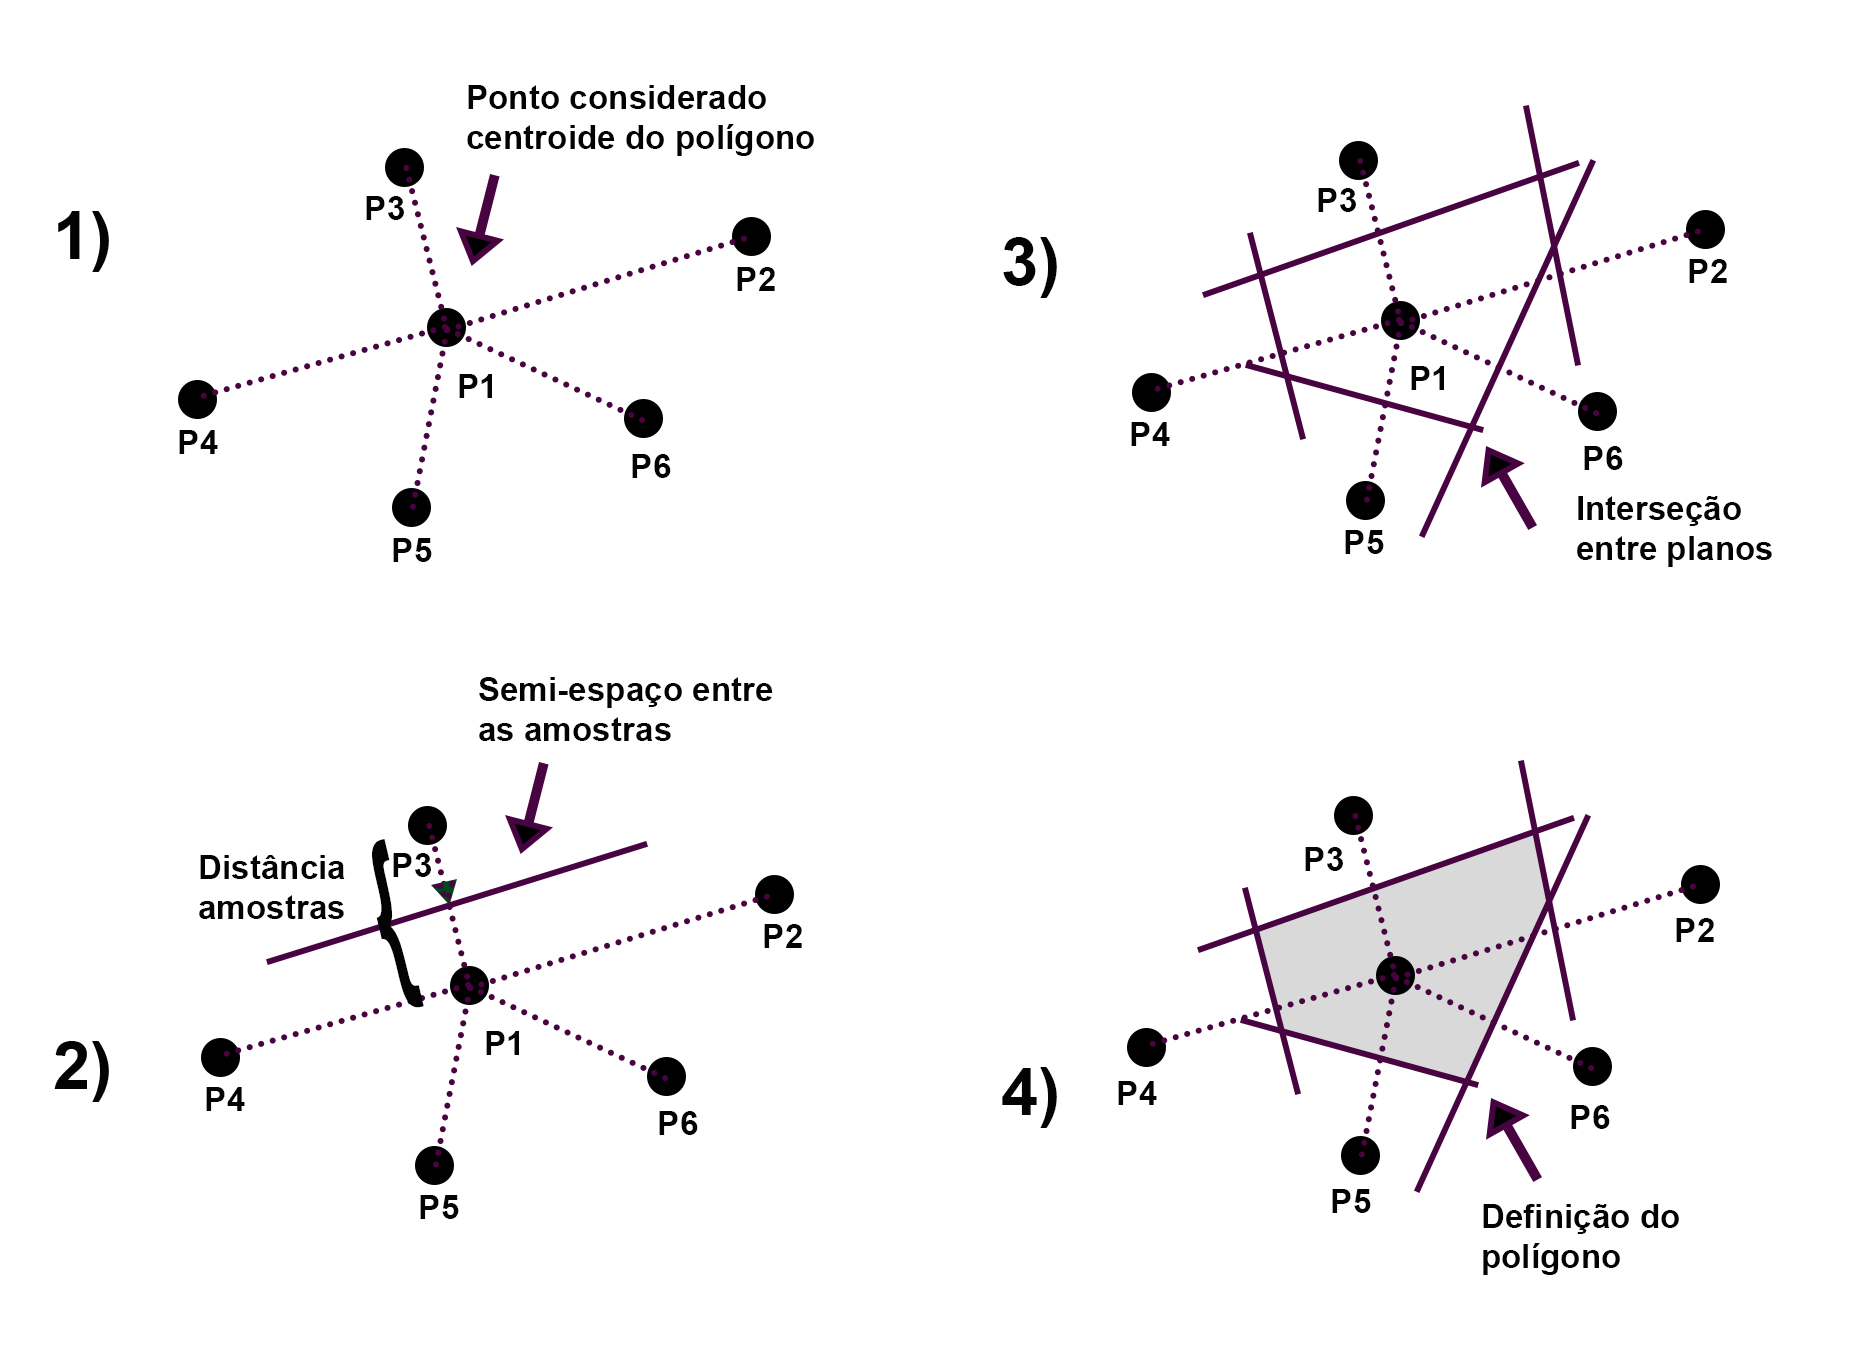
\includegraphics[scale=0.7]{./Capitulo_4/tpoligons.png}	
	\caption{4 etapas para a geração do polígono de Tiessen a partir de um ponto amostral considerado centroide $(P_{1})$. 1) Determinar o ponto amostral considerado centroide do polígono. Unir aos pontos mais próximos semi-retas ligando o centroide. 2) Determinar os semi-planos formados pela reta perpendicular as semi-retas que ligam o centroide pela metade da distância entre eles. 3) Determinar os vértices do polígono a partir da interseção entre as retas determinadas no item 2. 4)Ligar todos os vértices do polígono. A solução é única e gerará um polígono convexo.  }
	\label{tiessen}
\end{figure}
\FloatBarrier 

\begin{proposition}
	\textit{A solução por polígonos de Tiessen é puramente geométrica. Nenhuma consideração é feita sobre a relação entre as propriedades de uma amostra no espaço. Apenas é realizada a extensão desta propriedade para uma área considerada de influência da amostra.} 
\end{proposition}

Os polígonos de Tiessen possuem alugumas propriedade geométricas. O vértice de um polígono de Tiessen é correspondente ao centro geométrico do círculo formado pelo centroide do polígono e dois pontos mais próximos. A figura  \ref{tiessen2} apresenta esta propriedade. Ao unir triângulos entre os pontos mais próximos é criada a chamada \textbf{tesselação de Delunay}, em que o baricentro do triângulo é também correspondente ao vértice do polígono de Tiessen. 

 

\FloatBarrier
\begin{figure}[!htpb]
	\centering
	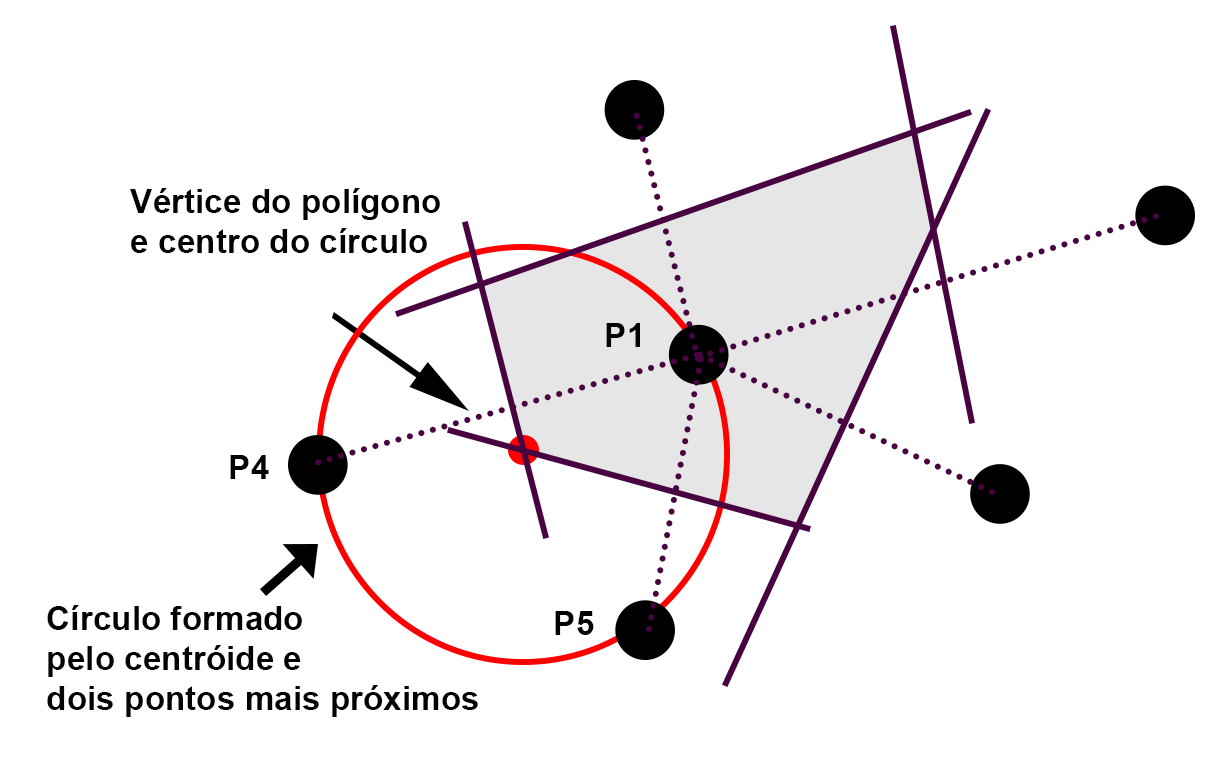
\includegraphics[scale=0.9]{./Capitulo_4/propTy.png}	
	\caption{Propriedade dos polígonos de Tiessen. Centro do círculo composto pelo baricentro e dois pontos mais próximos forma um vértice do polígono de Tiessen.}
	\label{tiessen2}
\end{figure}
\FloatBarrier 

É comum para os pontos que se situam nas extremidades do conjunto de dados não possuirem uma solução de polígono fechado, como ocorre nos pontos amostrais interiores. Neste caso geralmente se forma uma extrapolação da área de influência. Esta extrapolação pode considerar quesitos geológicos ou puramente geométricos, mas é um critério muito mais subjetivo que indicativo. A figura \ref{tiessen3} apresenta esta extrapolação. 

\FloatBarrier
\begin{figure}[!htpb]
	\centering
	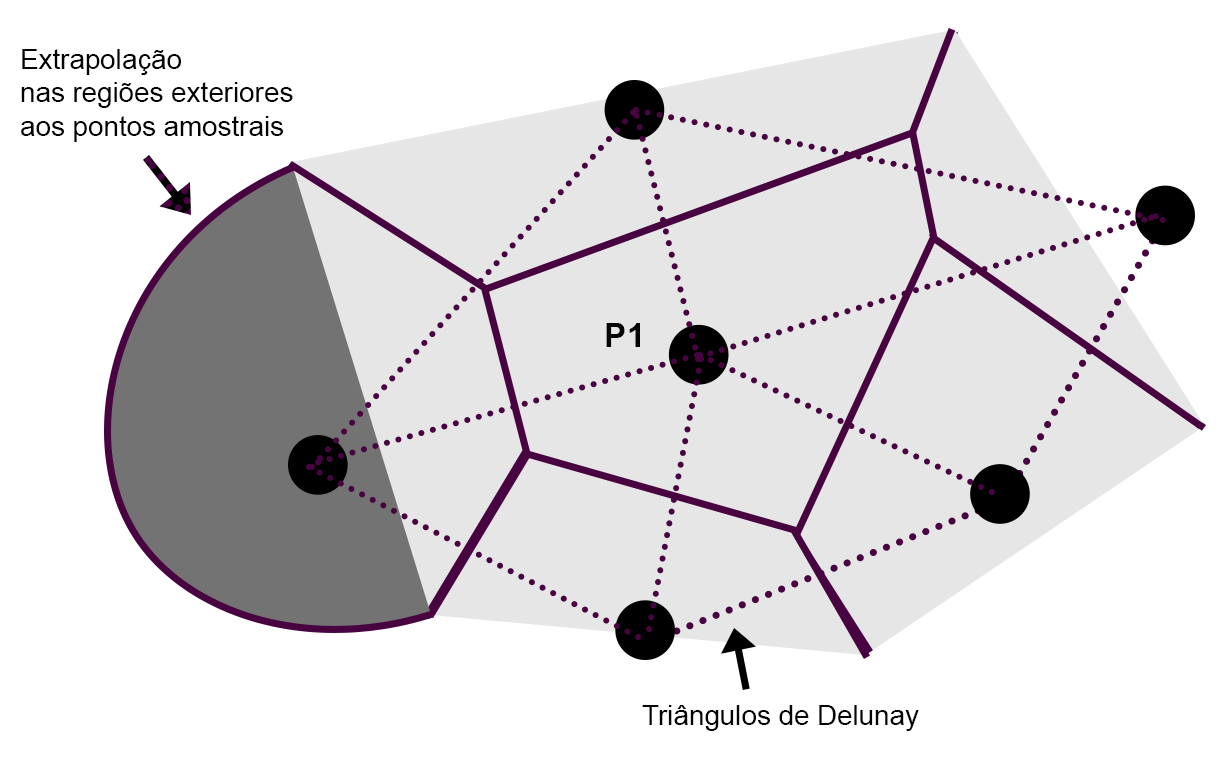
\includegraphics[scale=0.9]{./Capitulo_4/tyssen4.png}	
	\caption{Extrapolação realizada nos pontos amostrais situados na extremidade. Extrapolação apresentada pelo um arco de cor cinza escuro.}
	\label{tiessen3}
\end{figure}
\FloatBarrier 

Para obter o teor médio do depósito a partir dos polígonos de Tiessen basta considerar a média ponderada entre as áreas de influência, tal como na equação 


\begin{equation} \label{pondemed} 
t_{m} = \frac{\sum_{i=1}^{n} A_{i}t_{i}}{\sum_{i=1}^{n} A_{i}}
\end{equation}

Em que $A$ representa a área do polígono de Tiessen para cada ponto amostral $i$ e $t$ representa o teor da área representado pelo valor da amostra em seu centroide. A solução tridimensional para os polígonos de Delunay é os chamados poliedros de Delunay. A solução tridimensional é complicada, e geralmente envolve elementos de topologia de alto nível computacional e matemático. A simplificação utilizada é utilizar o princípio do vizinho mais próximo, dividindo o espaço em uma malha de tamanho infinitesimal e atribuindo em cada célula a propriedade do ponto amostral mais próximo. Quando o tamanho da célula tende a um valor infinitesimal a solução pelo vizinho mais próximo converge para os polígonos ou poliedros de Tiessen. A figura \ref{tiessen3} representa um mapa dos polígonos de Tiessen a partir do método do vizinho mais próximo e uma maha de tamanho unitário.

\FloatBarrier
\begin{figure}[!htpb]
	\centering
	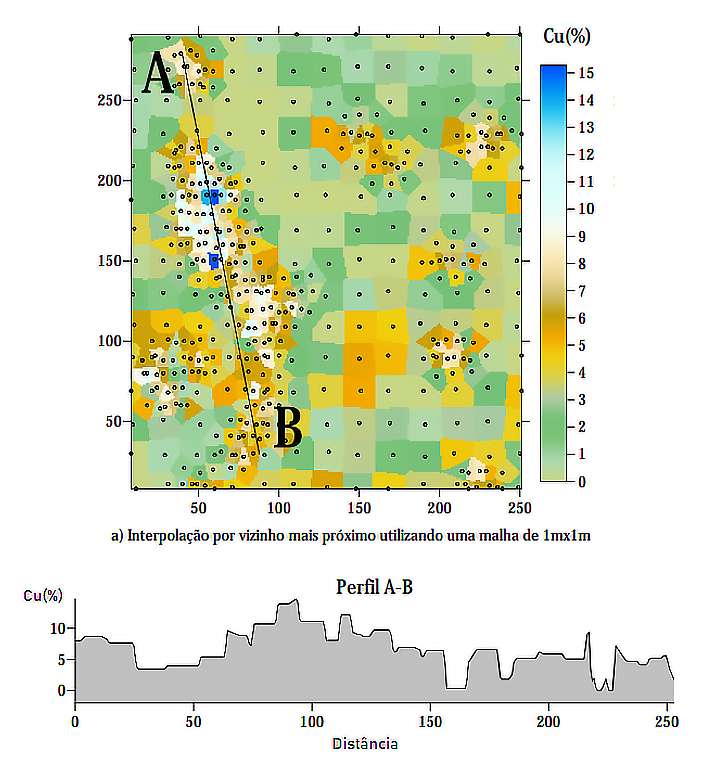
\includegraphics[scale=0.50]{./Capitulo_4/nearest.png}	
	\caption{Aproximação dos polígonos de Thiessen a partir do vizinho mais próximo, utilizando uma malha de 1mx1m}
	\label{tiessen3}
\end{figure}
\FloatBarrier 

\section{Estatísticas desagrupadas} \label{demons_krig} 

As malhas de amostragem representam uma importante fonte de informação para a realização dos métodos geoestatísticos. O posicionamento das amostras caracteriza a informação espacial a ser representada pelos métodos de estimativa. Quando pensamos em termos de representatividade a amostragem regular no espaço é a que melhor representa as características do depósito mineral. Em alguns casos é possível distribuir a malha segundo a continuidade espacial do depósito, permitindo um maior afastamento nas regiões mais contínuas do depósito e menos espaçadas nas regiões menos contínuas. A figura \ref{malhas}[A] apresenta esquematicamente uma malha regular e irregular. Em \ref{malhas}[B] é apresentado a disposição da malha segundo a continuidade do corpo geológico.

\FloatBarrier
\begin{figure}[!htpb]
	\centering
	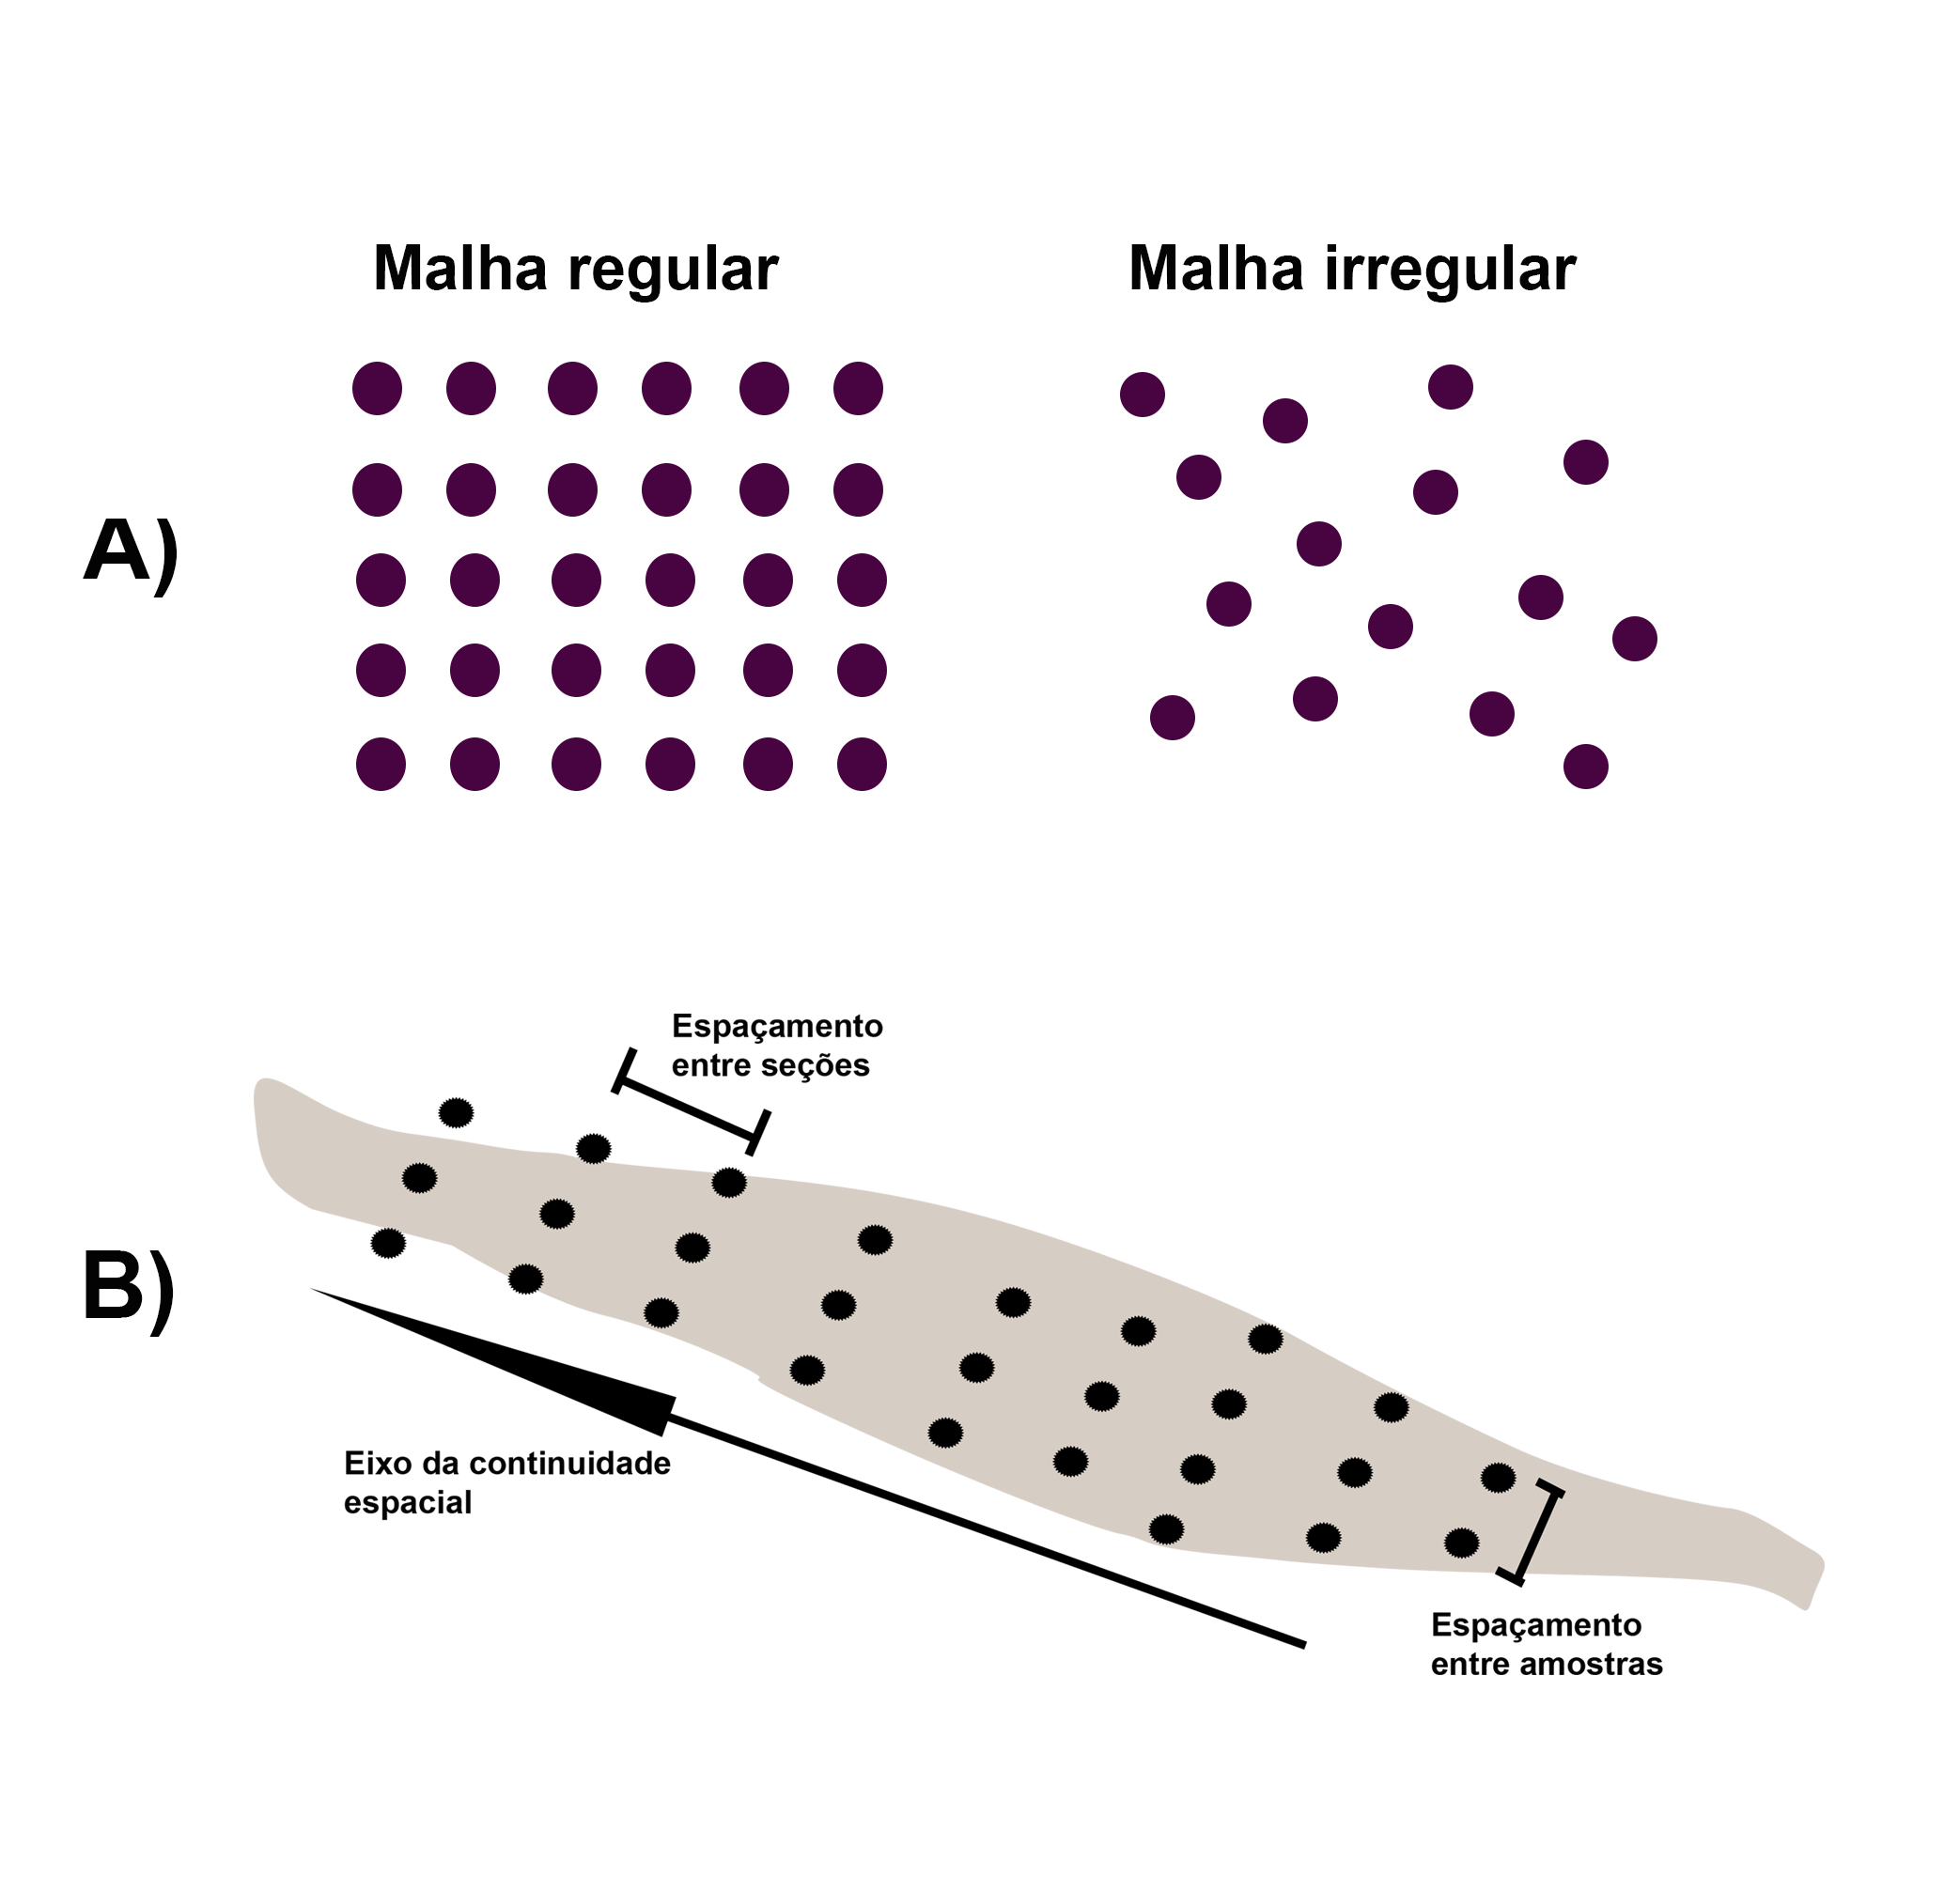
\includegraphics[scale=0.6]{./Capitulo_4/malhas.png}	
	\caption{A) Representação de uma malha de amostragem regular e uma malha de amostragem irregular B) disposição de amostras segundo a continuidade espacial do corpo geológico.}
	\label{malhas}
\end{figure}
\FloatBarrier 

Nos problemas de engenharia geológica, a disposição das malhas de sondagem dependem de diversos fatores, como por exemplo, terrenos de maior declividade que impedem a utilização de sondas, áreas de proteção ambiental, regiões de córregos ou outros fatores que podem impedir a formação de uma malha regular. Além disso, pela natureza de risco da atividade econômica, é comum adensar amostragens em lugares específicos onde possuam maior interesse para a mineração, como teores metálicos mais altos, ou litotipos de maior importância. Isto forma um agrupamento ou \textit{cluster}. A figura \ref{posicionamento} apresenta esquematicamente a formação de um agrupamento nas amostras.

\FloatBarrier
\begin{figure}[!htpb]
	\centering
	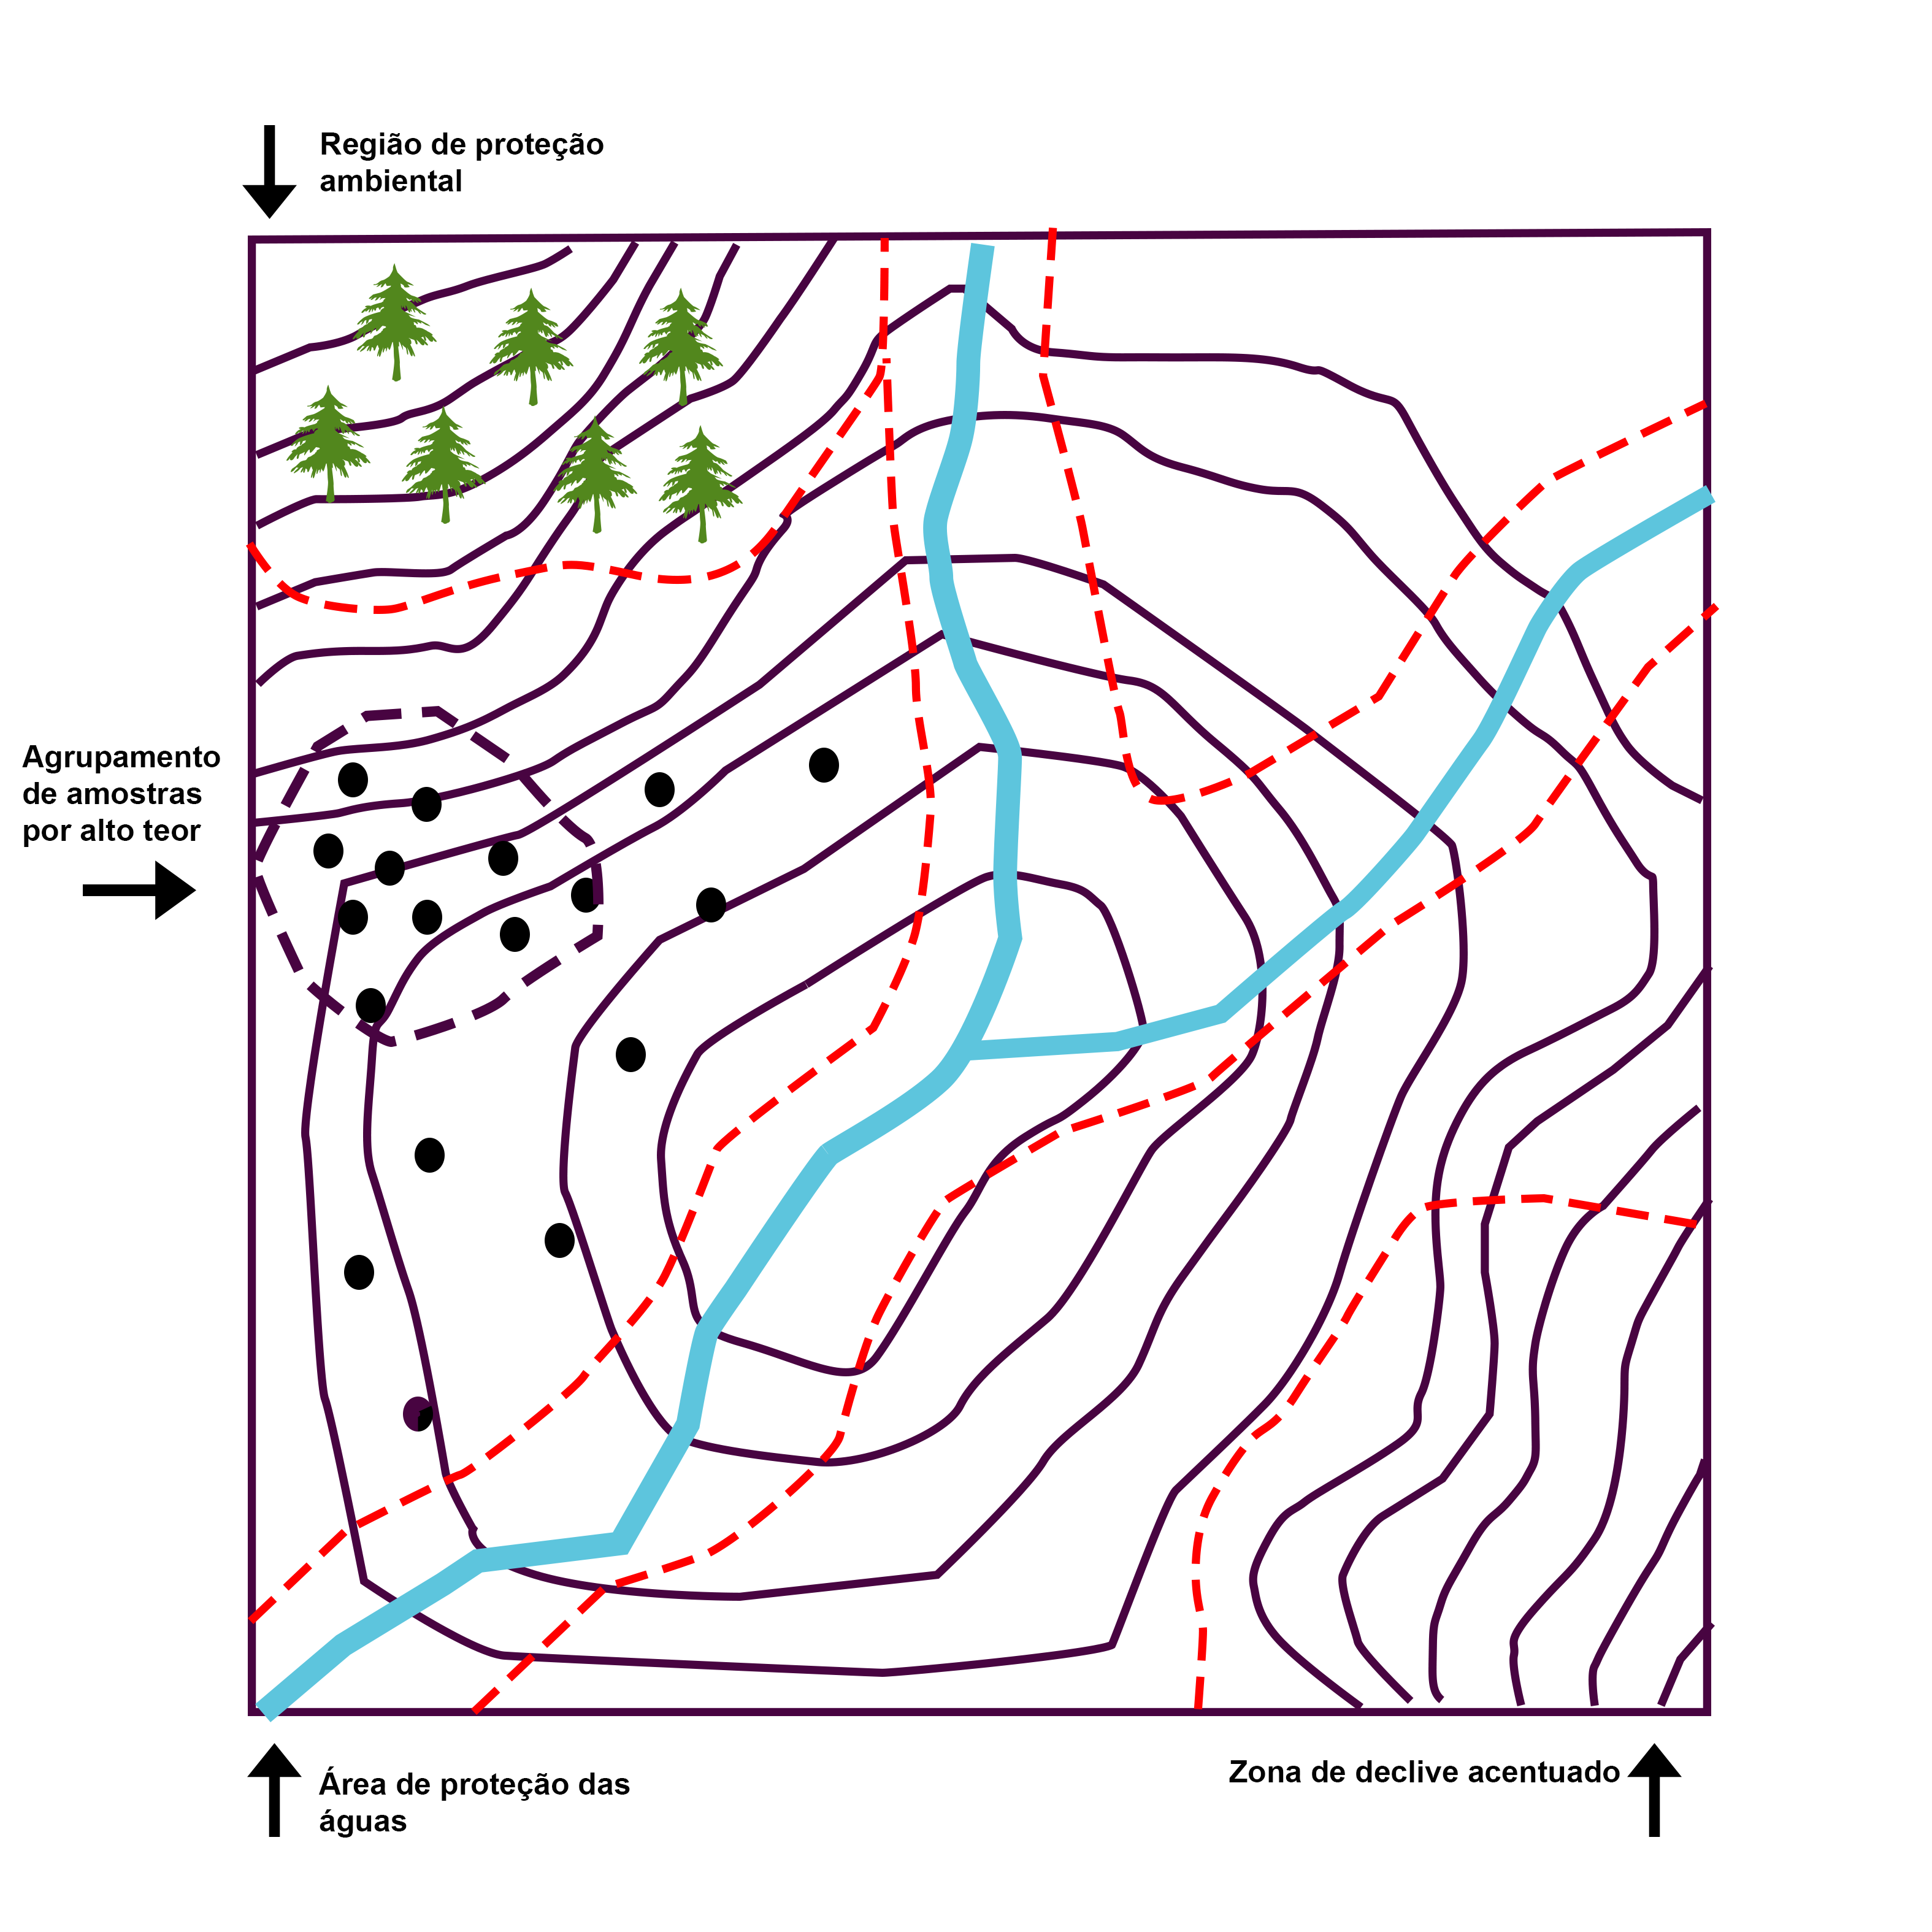
\includegraphics[scale=0.4]{./Capitulo_4/posicionamento.png}	
	\caption{Representação de uma área amostrada. Obstáculos para a amostragem representados pela presença de áreas de preservação, terreno com maiores inclinações e área de reservas hídricas. Amostragem irregular realizada a oeste do desenho do mapa.}
	\label{posicionamento}
\end{figure}
\FloatBarrier 

Calcular estatísticas considerando apenas os dados sem sua disposição espacial pode resultar em enviesamento. Se muitas análises são realizadas apenas em locais onde ocorre alto teor, os resumos estatísticos produziram também resultados com alto valor, mesmo que eles não correspondam à representação do domínio de estimativa. 

\begin{remark}
	\textit{"É natural que os dados georeferenciados coletados são de uma forma não representativos. Amostragens preferenciais em áreas de interesse são intencionais e facilitadas pela intuição geológica, dados análogos e amostragens anteriores. A prática de coletar amostras agrupadas ou espacialmente enviesadas é encorajada pelas restrições técnicas e econômicas, tal como produções futuras, acessibilidade e custos de análise dos laboratórios"} -\cite{pyrcz2003declustering}
\end{remark}

Um dos maiores erros cometidos por iniciantes ao considerar o desagrupamento de amostras é substituir os valores das amostras pelos valores dos pesos de desagrupamento. A alteração realizada pelo desagrupamento deve ser feita apenas sobre as estatísticas e não sobre seu valor bruto. 

\begin{definition}[Desagrupamento]
	\textit{Dada uma estatística $\phi(Z)$ a partir de uma variável aleatória $Z$, uma estatística desagrupada $\theta$ é aquela que pode ser aplicada de tal forma que $\theta(\phi(Z))$ considerando as distâncias euclidianas relativas entre as amostras.}  
\end{definition}


As duas principais técnicas utilizadas para desagrupamento são os polígonos de influência, ou de Tiessen vistos anteriormente e o desagrupamento por células.





\subsection{Polígonos de influência} 

O desagrupamento das amostras pode ser realizado a partir de áreas de influência como no caso dos polígonos de Thiessen. A frequência de cada valor pode ser alterada pela área do polígono respectivamente. Observe a figura \ref{tissen_hist}. Cada ponto amostral $\{P_{1},P_{2},P_{3},P_{4},P_{5}, P_{6} \}$ possui uma área gerada pelo vizinho mais próximo em um grid de tamanho de célula conhecida. Abaixo podemos ver um histograma representando a frequência destes pontos. Se consideramos apenas seus valores brutos, e não sua disposição espacial, cada ponto assume um valor de frequência igual a 1. No caso da utilização das áreas pelos polígonos  

\FloatBarrier
\begin{figure}[!htpb]
	\centering
	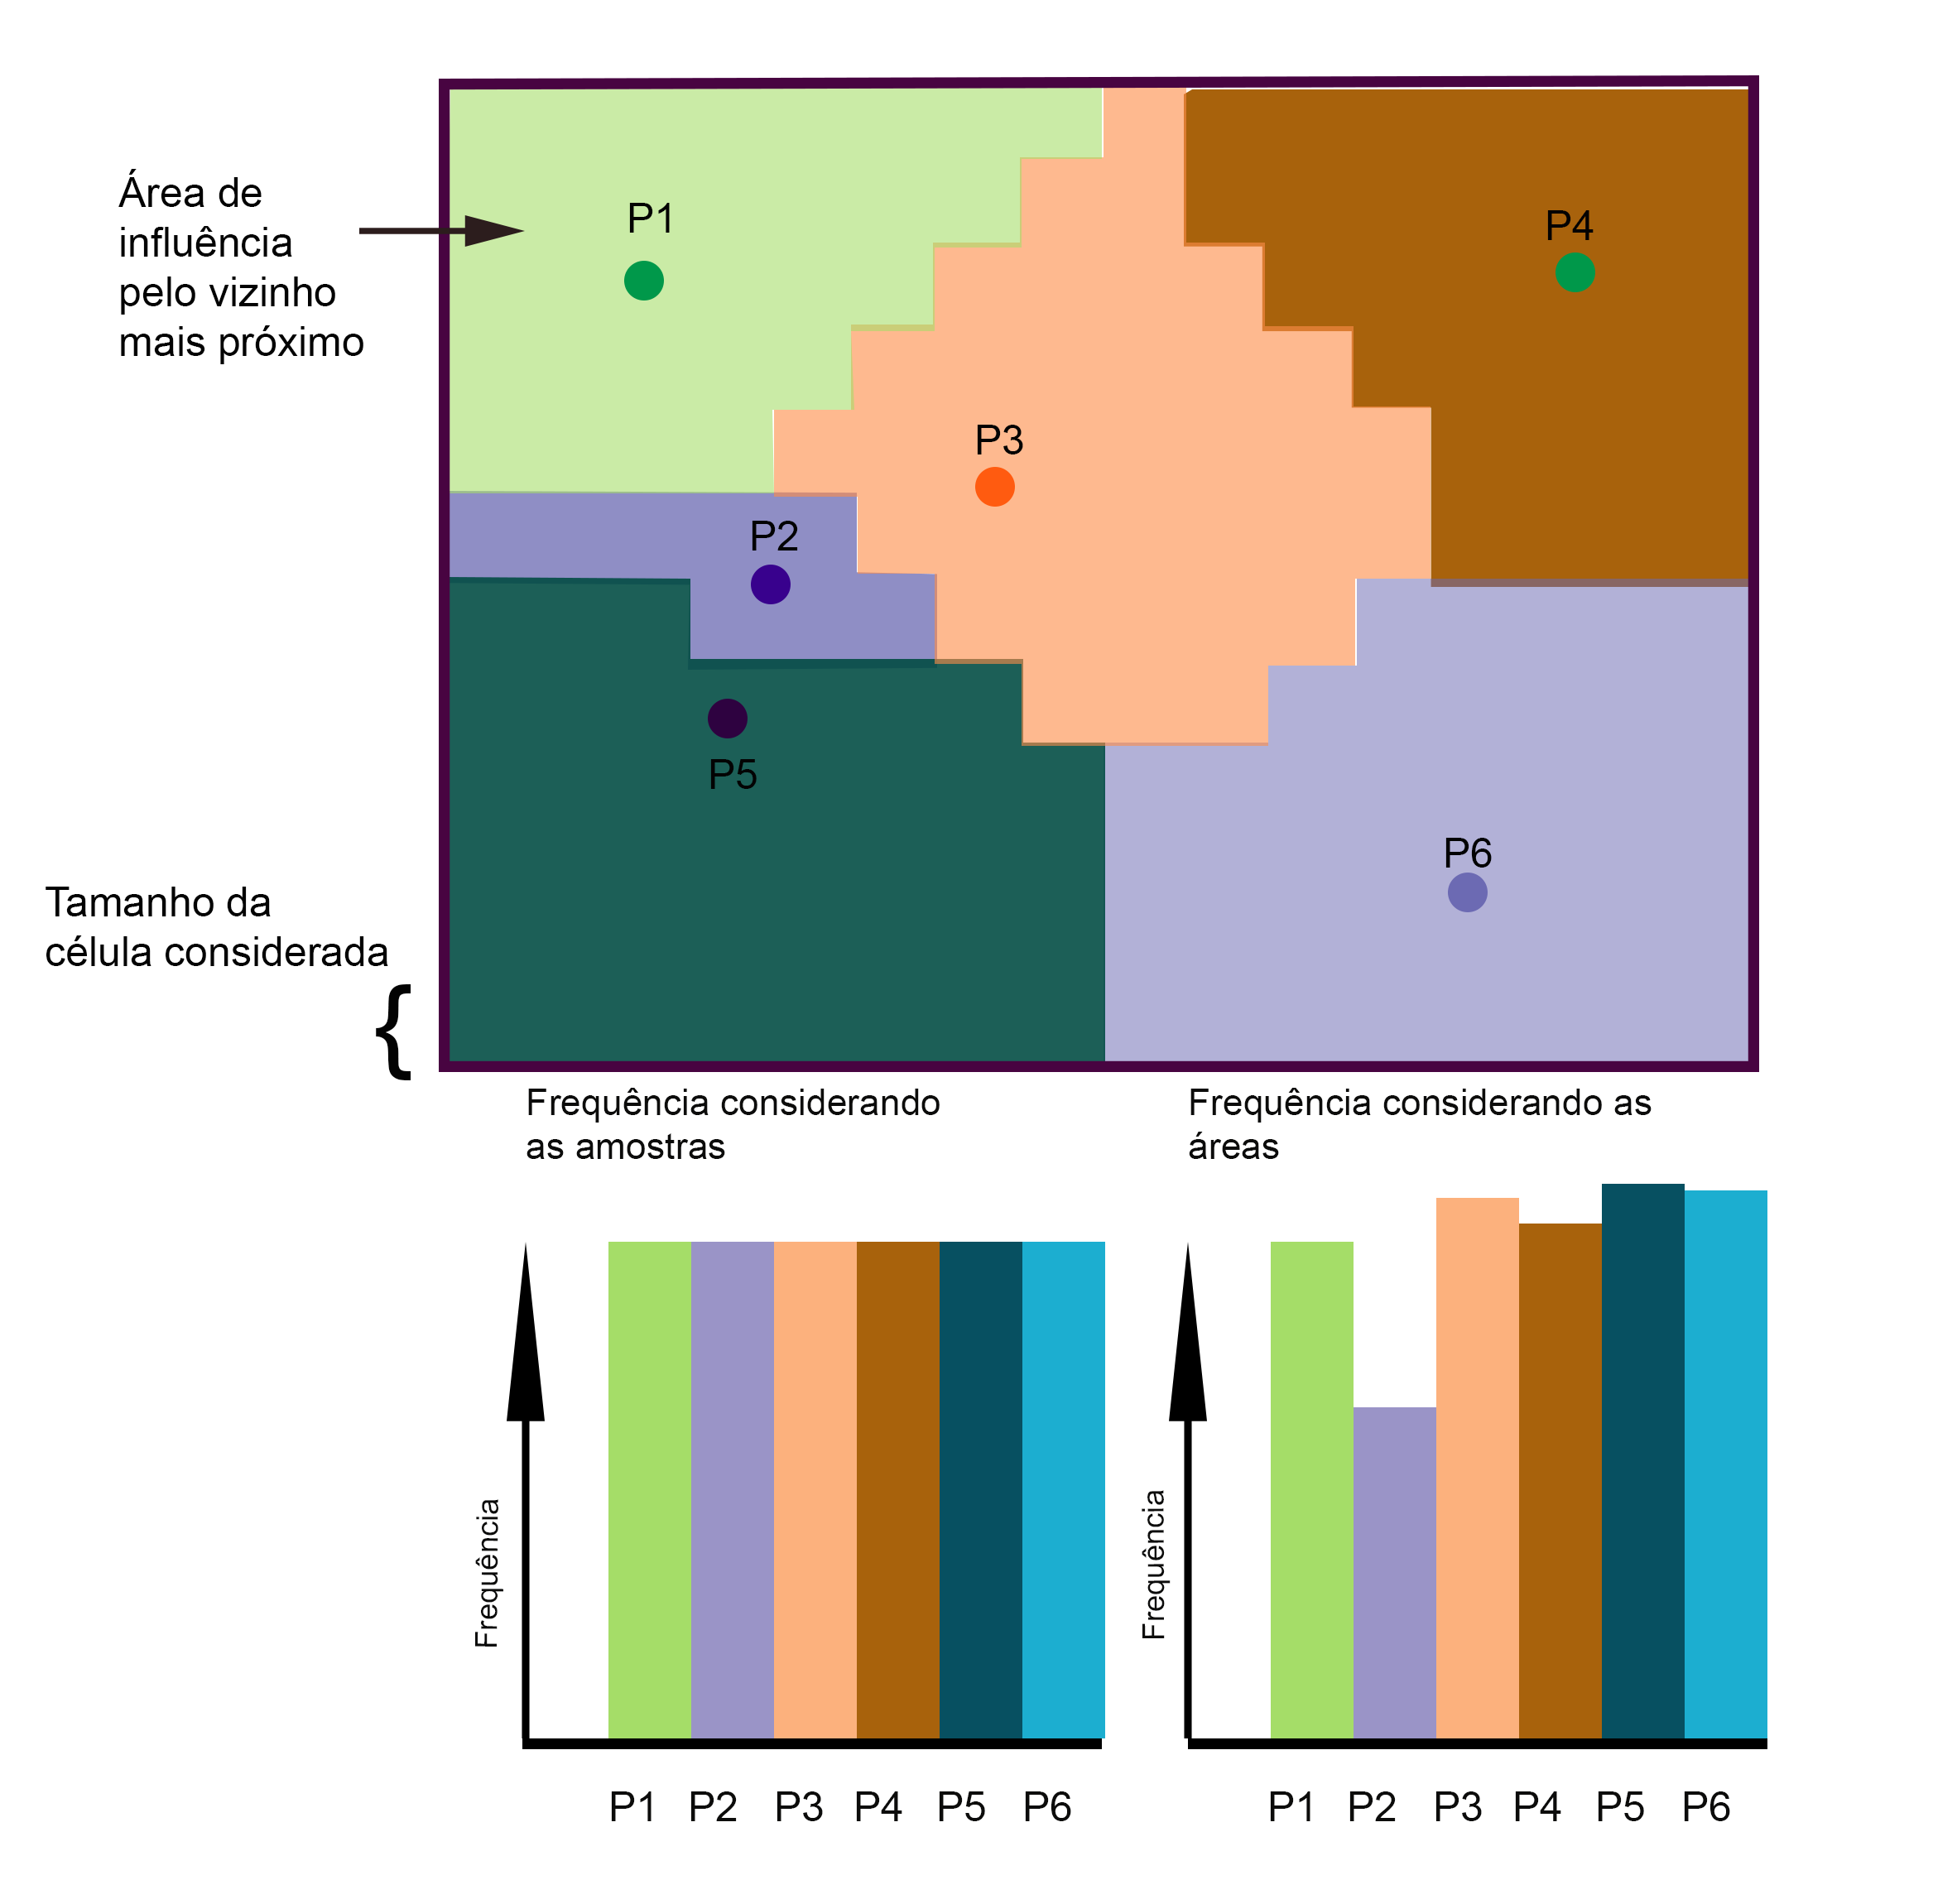
\includegraphics[scale=0.7]{./Capitulo_4/ponderacao.png}	
	\caption{Representação de uma área amostrada. Obstáculos para a amostragem representados pela presença de áreas de preservação, terreno com maiores inclinações e área de reservas hídricas. Amostragem irregular realizada a oeste do desenho do mapa.}
	\label{tissen_hist}
\end{figure}
\FloatBarrier 

\begin{definition}[Desagrupamento por polígonos de influência]
	\textit{Dado uma amostra $Z$ com uma realização $z$,  $F(Z=z)$ representa a frequência de um elemento da amostra. Logo $F(Z=z) = A(z)$, sendo $A(z)$ a área de influência de um elemento $z$ da amostra. }  
\end{definition}

\subsection{Desagrupamento por células} 

O desagrupamento realizado por polígonos de influência, gera uma solução única, e não permite encontrar pesos diferentes para as amostras, no entanto, o método de desagrupamento por células é flexível, permitindo ajustar parâmetros que indicarão o melhor resultado. O método considera a divisão do espaço em 'células' de mesma dimensão, tal que  o peso de cada amostra é dado pelo número de amostras contidas dentro de cada célula. Observe a figura \ref{cel_declus}. A célula da linha 1 e coluna 1 apresenta apenas duas amostras, o que significa que cada uma receberá um peso de 1/2. 

\FloatBarrier
\begin{figure}[!htpb]
	\centering
	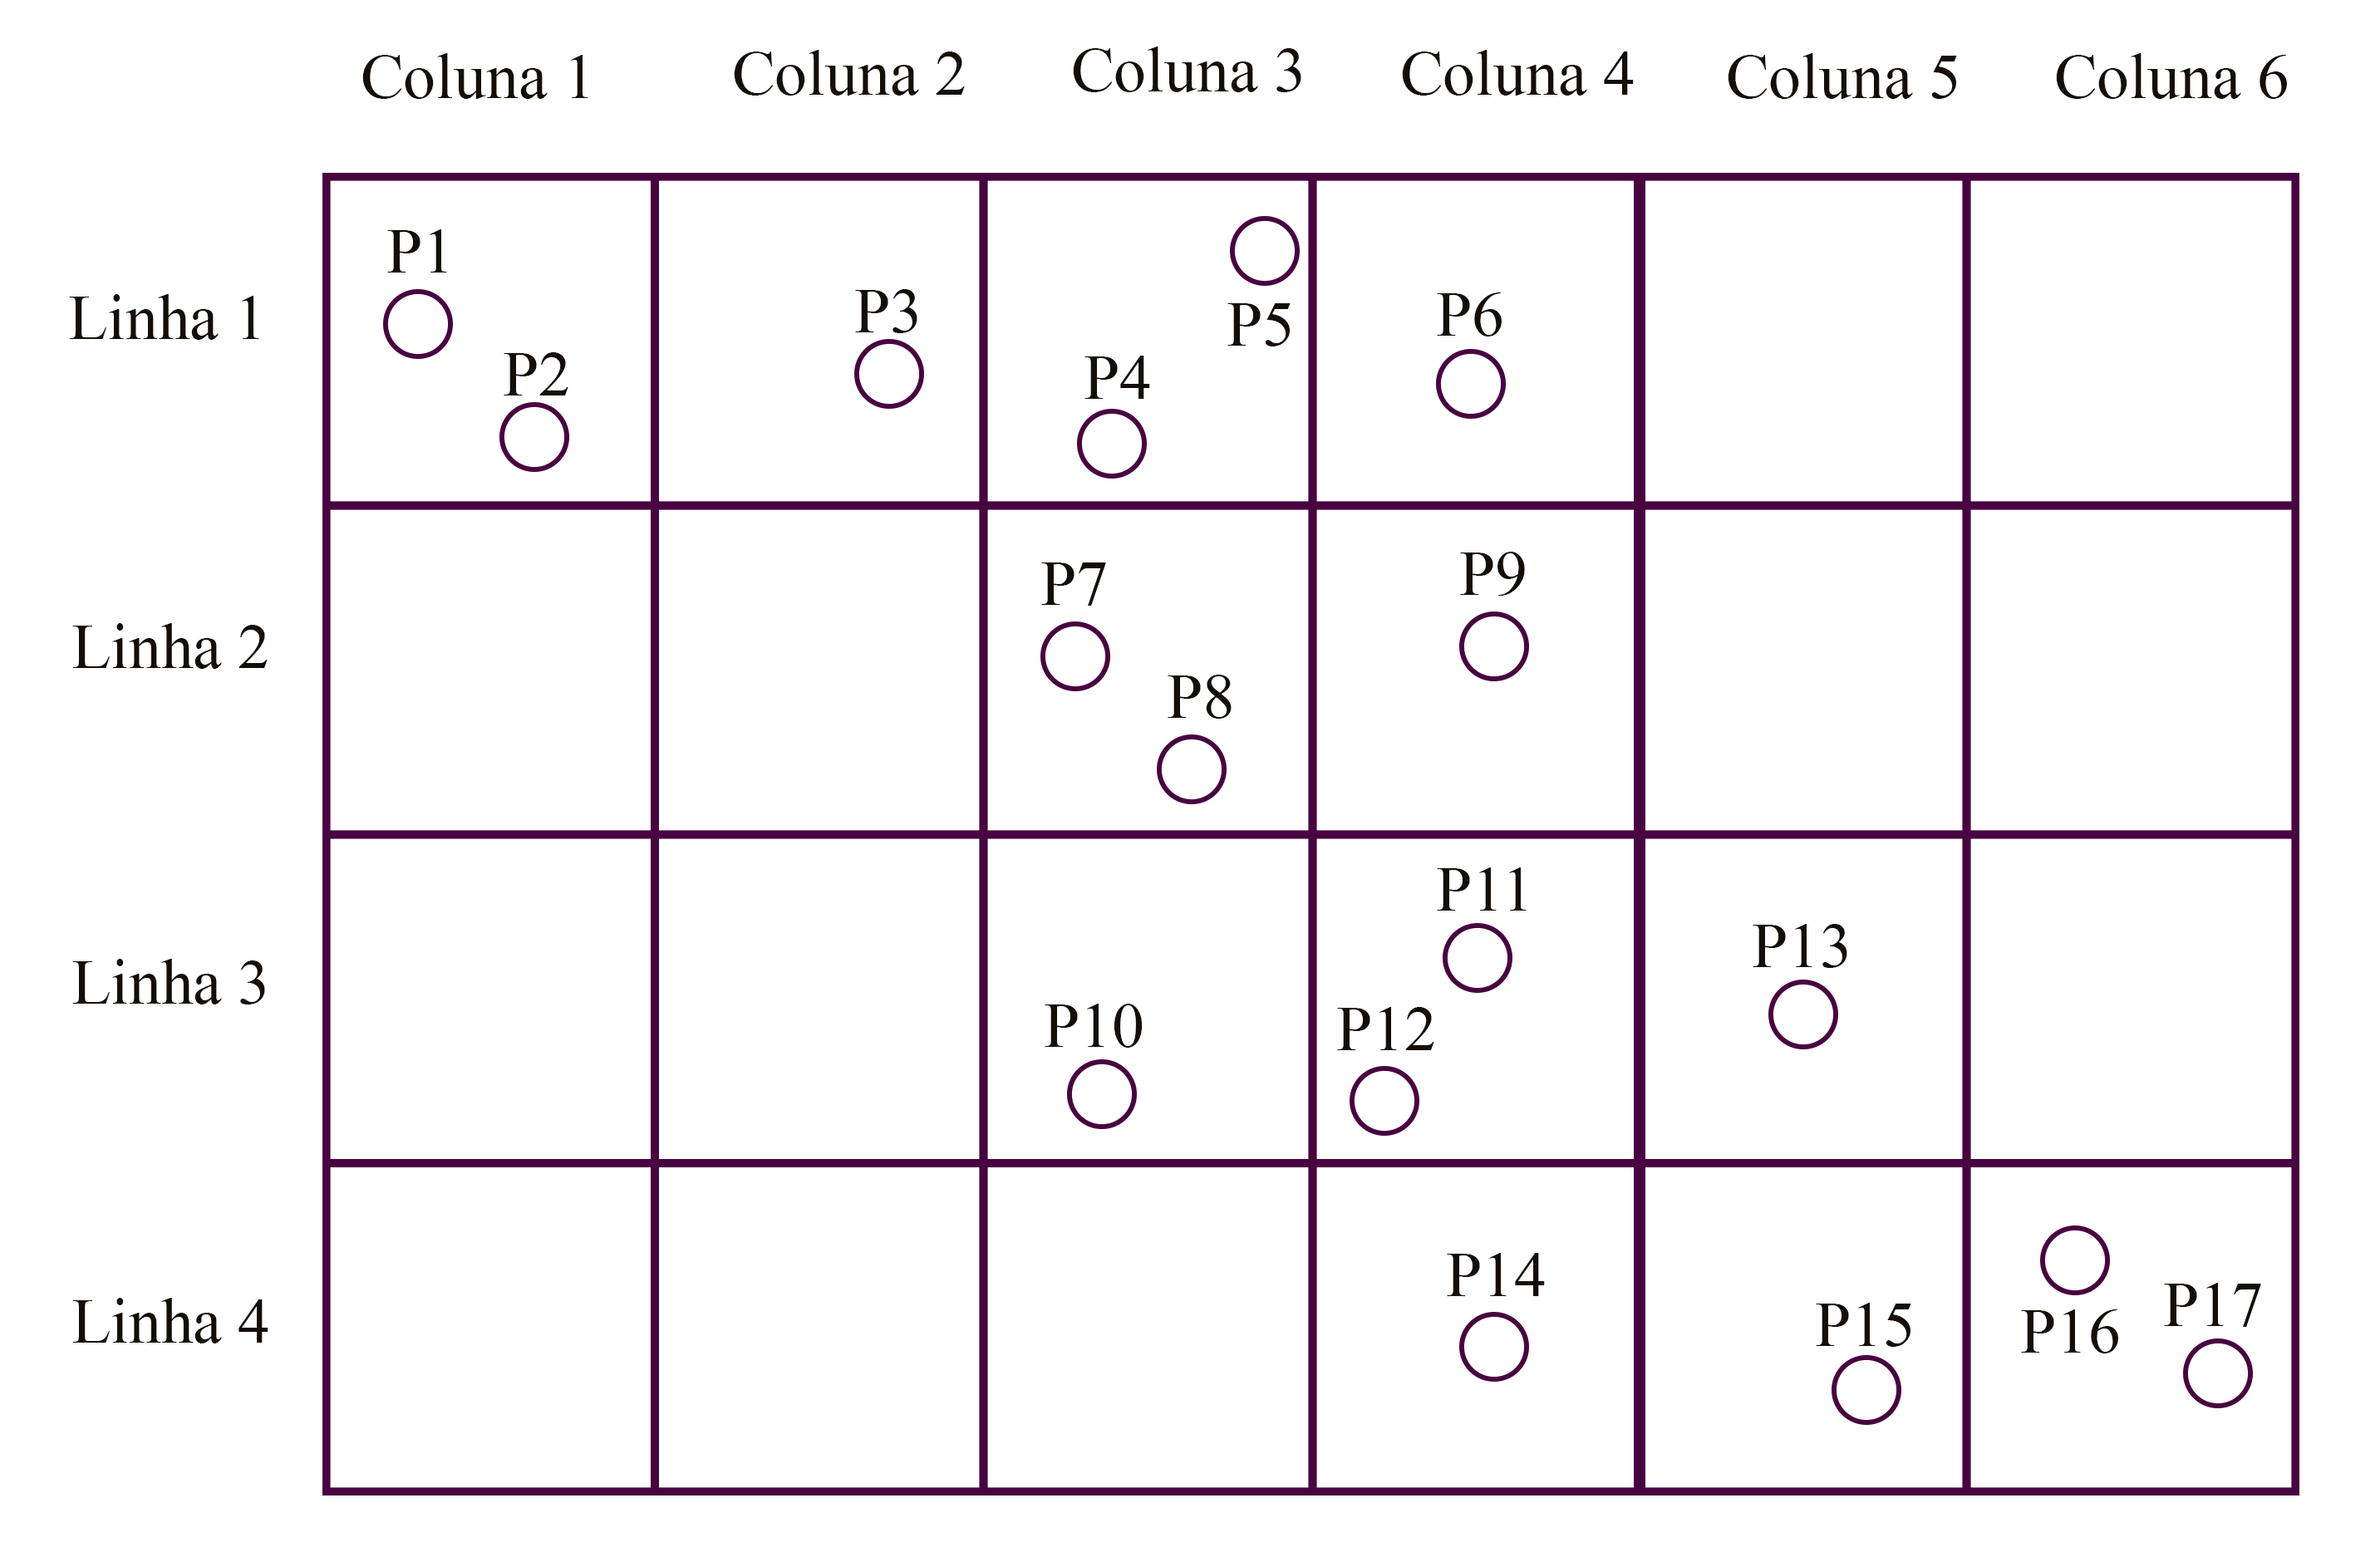
\includegraphics[scale=0.1]{./Capitulo_4/desagrupamento_celula.png}	
	\caption{Representação do desagrupamento das células em um espaço bidimensional.}
	\label{cel_declus}
\end{figure}
\FloatBarrier 

Evidentemente o tamanho da célula definirá o peso do desagrupamento. Uma célula muito grande que ocupe toda a extensão territorial analisada terá peso idêntico a $1/n$, sendo o n o número de amostras. Logo o ponderador das amostras será igual a equação \ref{pondemeded} 

\begin{equation} \label{pondemeded} 
p_{t_{i}} = (1/n)/\left(\sum_{i=1}^{n}1/n\right) = 1/n
\end{equation}

Exatamente igual a média aritmética dos valores. Da mesma forma se forem escolhidos tamanhos de células tão pequenas que apenas uma amostra esteja contida, teremos um valor de peso igual a 1, também obtendo o valor da média aritmética. A escolha do tamanho da célula deve ser feita entre estes dois casos extremos, aos quais teremos o menor valor desagrupado da média.
 A figura \ref{cel_declus_graf} demonstra a procura do tamanho da célula quadrada mais próxima do menor valor da média desagrupada, definindo assim o resultado que pretendemos. 

\FloatBarrier
\begin{figure}[!htpb]
	\centering
	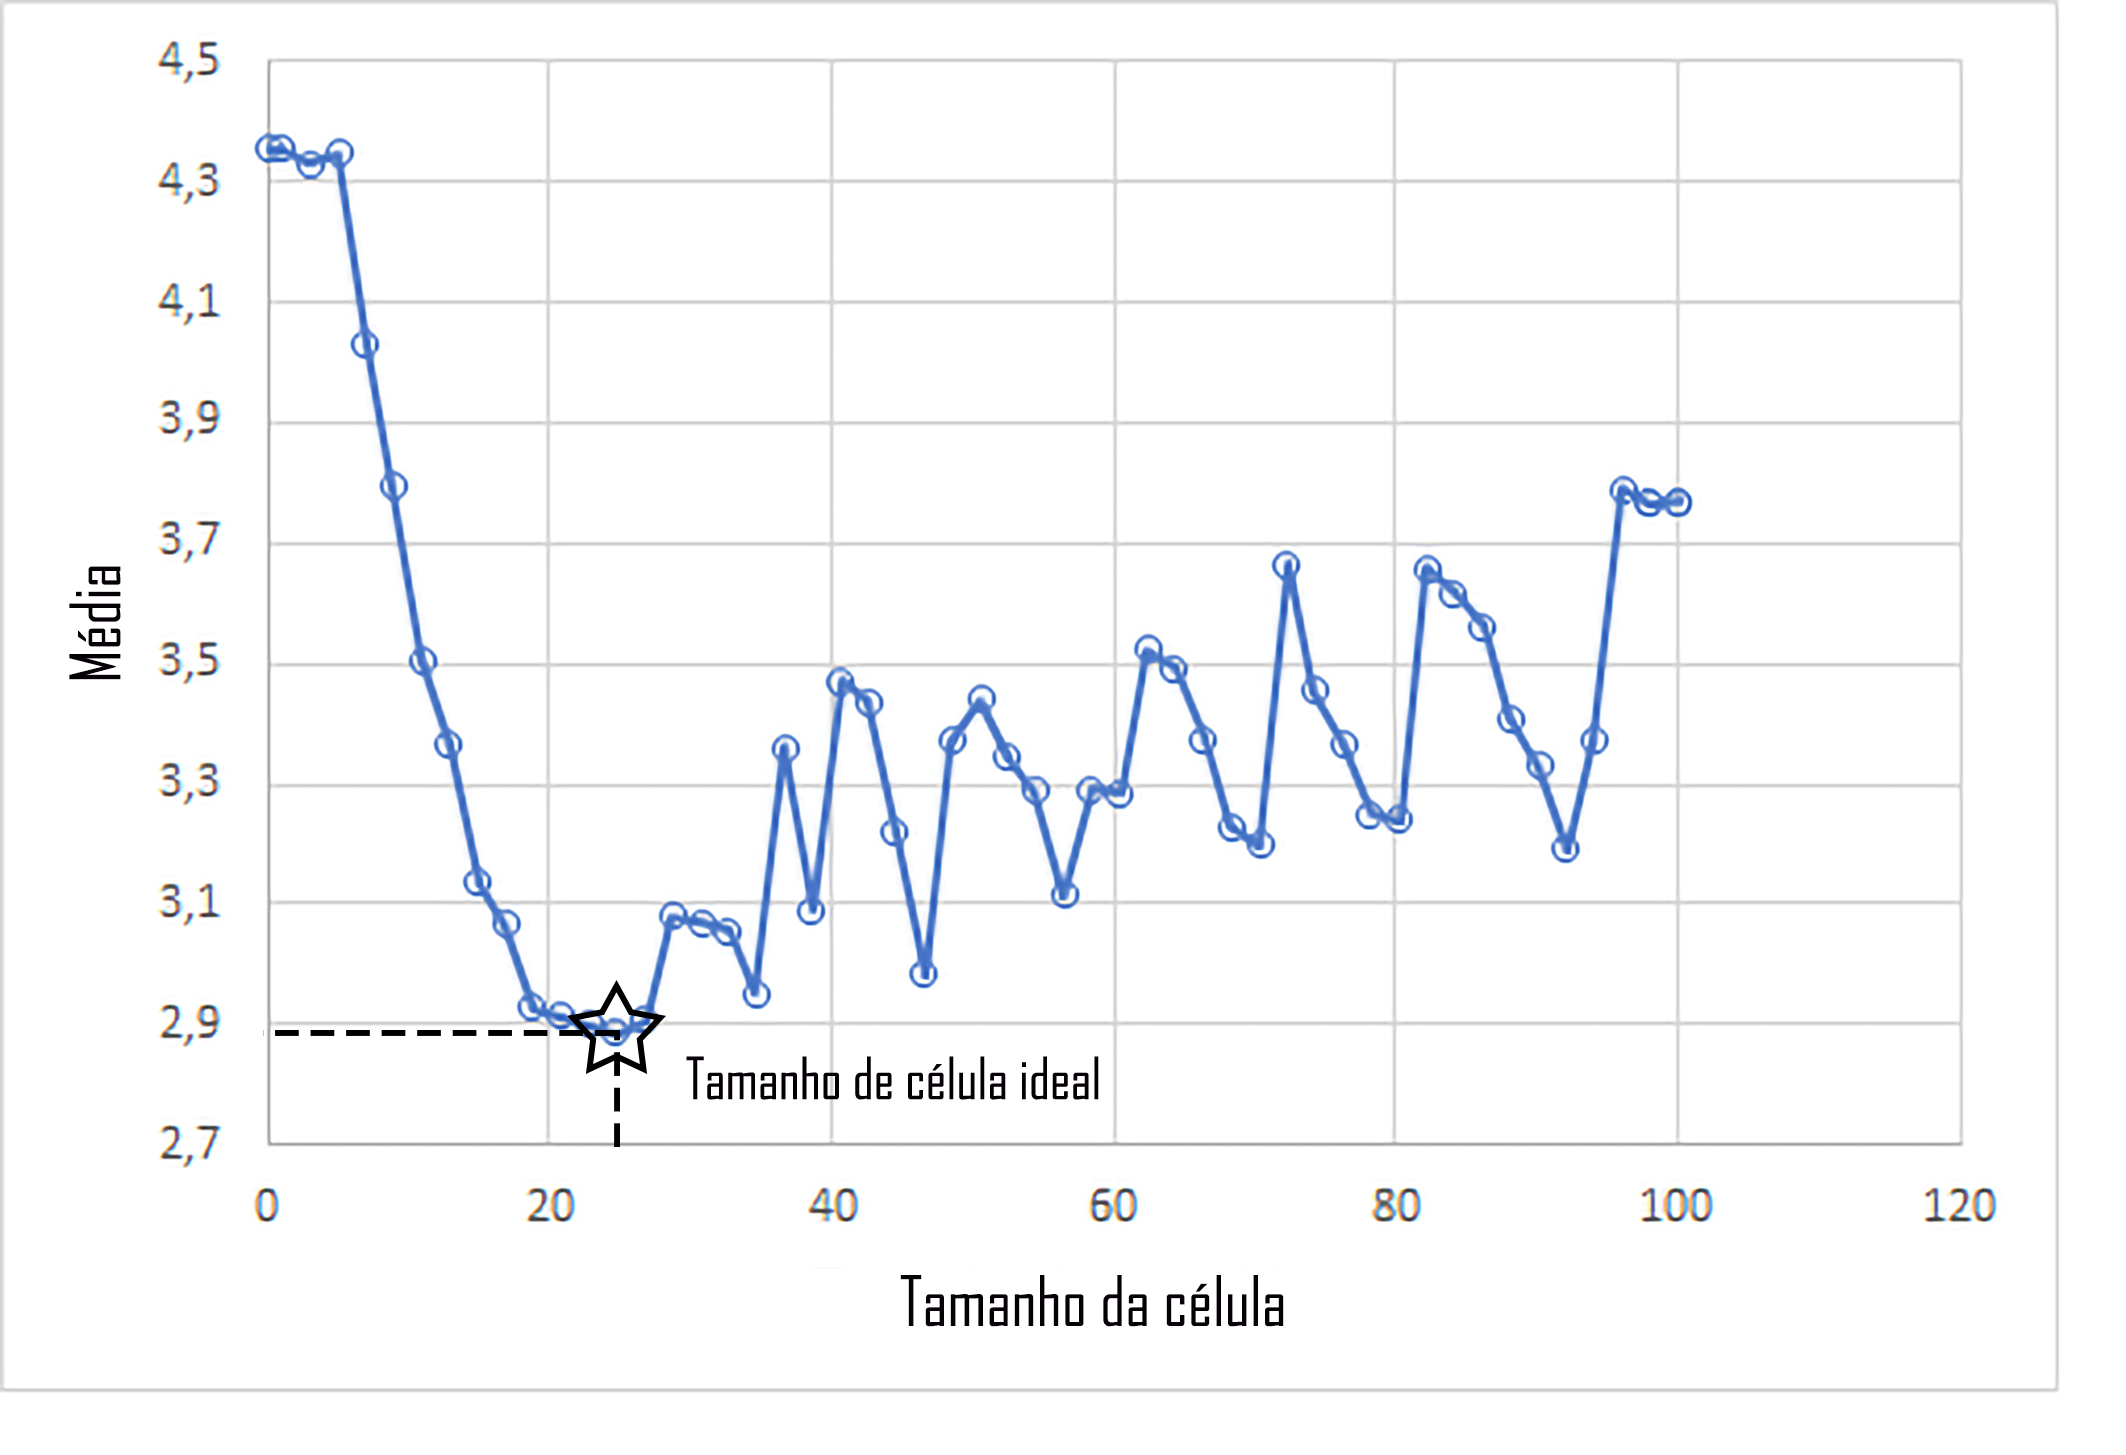
\includegraphics[scale=0.18]{./Capitulo_4/desagrupamento_celula_graf.png}	
	\caption{Representação da escolha do melhor tamanho de célula dado um conjunto de médias desagrupadas.}
	\label{cel_declus_graf}
\end{figure}
\FloatBarrier 


\begin{exercise}
	Os dados da tabela abaixo representam um conjunto de amostras bidimensionais, em que x e y representam respectivamente as coordenadas cartesianas nos eixos das abicissas e das ordenadas. Para a configuração geométrica abaixo, determine os polígonos de Thyssen, e consequentemente os ponderadores para cada uma das amostras. (Obs.: Feche os polígonos no limite exterior da região das amostras ligando diretamente as amostras) 
	
	\centering
	\begin{tabular}{lllll}
		\hline
		x & y  & z    &  &  \\ \hline
		1 & 2  & 1.09 &  &  \\
		1 & 3  & 0.50 &  &  \\
		1 & 4  & 2.01 &  &  \\
		2 & 3  & 2.04 &  &  \\
		2 & 7  & 7.90 &  &  \\
		3 & 4  & 3.05 &  &  \\
		3 & 5  & 2.02 &  &  \\
		3 & 9  & 3.04 &  &  \\
		4 & 5  & 2.01 &  &  \\
		4 & 7  & 2.01 &  &  \\
		4 & 10 & 3.07 &  &  \\ \hline
	\end{tabular}


\vspace{50px}
\centering
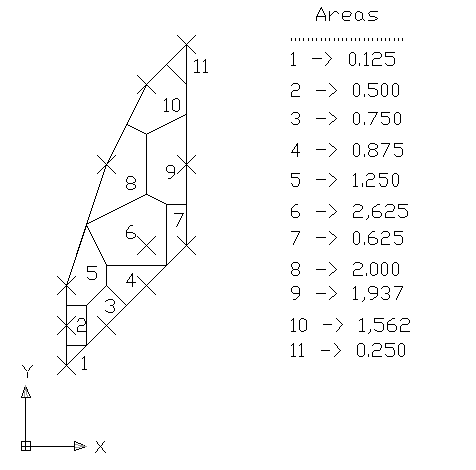
\includegraphics[scale=0.8]{./Capitulo_4/area_influ.png}	

\end{exercise} 

\begin{exercise}
	Para os dados do exercício anterior encontre a média declusterizada e a variância declusterizada dos dados. 
\end{exercise}